%\documentclass[10pt,a4paper]{article}
%\usepackage[latin1]{inputenc}
%\usepackage{amsmath}
%\usepackage{amsfonts}
%\usepackage{amssymb}
%\author{}
%\title{}
%\begin{document}


\providecommand{\abs}[1]{\left\lvert#1\right\rvert}
\tableofcontents
\listoffigures
\pagebreak
\section{Introduction}

The study of two-particle correlations at low relative momentum is commonly known as femtoscopy.  Femtoscopic analyses are capable of measuring spatio-temporal characteristics of heavy-ion collisions, with a particular emphasis made on estimating the homogeneity lengths (also called radii) of the particle-emitting source.  These analyses traditionally study pions \cite{Goldhaber:1960sf,Aamodt:2011mr} because of their ready availability and sensitivity to the spatial scale of the source.  However, measurements of heavier particles such as kaons \cite{Abelev:2012ms} and baryons \cite{Gos:2007cj} can serve to complement the pion results.  One motivation for studying an assortment of heavier particles is to test the hydrodynamic prediction that radial flow should cause the source radii to scale with the transverse mass $m_{\mathrm{T}}$ of the particles \cite{Csorgo:1995bi,Lisa:2005dd}.

Baryon--(anti)baryon correlation functions are also useful in the study of final state interactions (FSI).  Measurements of scattering lengths of pairs such as p$\Lambda$ and $\Lambda\Lambda$ are of interest for rescattering calculations, and, in the latter case, for understanding the properties of neutron stars \cite{SchaffnerBielich:2008kb,Wang:2010gr}.  Baryon-antibaryon correlations allow for the study of annihilation processes.  It has been argued that annihilation in the hadronic rescattering phase should be taken into account when determining particle yields \cite{Werner:2012xh,Karpenko:2012yf,Steinheimer:2012rd}.  This annihilation should result in an anticorrelation in baryon-antibaryon correlation functions.  Results from these femtoscopic analyses may be able to provide insight into the $p/\pi^+$ ratio measured in experiments at the LHC, which falls short of thermal model expectations \cite{Preghenella:2012eu}. 

In this note, we present two-$\Lambda$ momentum correlation functions measured in PbPb collisions at $\sqrt{s_{NN}}=2.76$ TeV by the ALICE Collaboration.  Results are shown for $\Lambda\Lambda$, $\bar{\Lambda}\bar{\Lambda}$ and $\Lambda\bar{\Lambda}$ pairs. The $\Lambda\Lambda$ and $\bar{\Lambda}\bar{\Lambda}$ results are presented as candidates for preliminary status. The $\Lambda\bar{\Lambda}$ results were previously approved as a physics preliminary plot.  The motivation for $\Lambda$ baryon femtoscopy is to complement previous studies, as well as to probe the little-measured strong interactions of these baryons.

The primary effect seen in $\Lambda\bar{\Lambda}$ correlations should be strong final state interactions (FSI).  A suppression of the correlation function at low relative momentum ($k^*$) is expected due to interactions in the baryon-antibaryon annihilation channel.  Suppressions of this sort have also been seen in $p \bar{p}$ interactions \cite{Gos:2007cj}, though the effects of this channel in charged particle studies can be somewhat obfuscated by Coulomb enhancement effects in the same $k^*$ region.  Also discussed in this note are the main influences on $\Lambda\Lambda$ correlations --- strong FSI and Fermi-Dirac statistics.  A long-term goal of this study is to measure characteristics of the interaction potential of the $\Lambda$ baryons.  More specifically, the scattering length $f_0$ and effective radius $d_0$ of the interaction can be extracted from two-$\Lambda$ correlations. It should also be noted that the H-dibaryon may have two $\Lambda$ as one of its decay channels \cite{PhysRevLett.38.195}, though a recent study at ALICE has suggested that a $\Lambda\Lambda$ bound state is unlikely.  The study of $\Lambda$ momentum correlations at ALICE may some day provide further measurements of this phenomenon, though endeavors in this direction are too preliminary to report upon at this time.

\section{Data analysis}
\subsection{Data selection}
\label{sec:DataSelection}
The analysis was performed on 31 July, 2013 using AliRoot v5-04-64-AN. The data were from PbPb collisions at $\sqrt{s_{NN}}=2.76$  TeV taken from the LHC11h (AOD115) pass 2 reconstruction. Runs were selected if they were listed with a pass 2 global quality of 1 ("Good run") in the Run Condition Table. Approximately 66 million combined central, semi-central and minimum bias events were analyzed. The following runs were used, which comprise both the positive (++) and negative magnetic (--) field orientations:

170593, 170572, 170388, 170387, 170315, 170313, 170312, 170311, 170309, 170308, 170306, 170270, 170269, 170268, 170230, 170228, 170207, 170204, 170203, 170193, 170163, 170159, 170155, 170091, 170089, 170088, 170085, 170084, 170083, 170081, 170040, 170027, 169965, 169923, 169859, 169858, 169855, 169846, 169838, 169837, 169835, 169591, 169590, 169588, 169587, 169586, 169557, 169555, 169554, 169553, 169550, 169515, 169512, 169506, 169504, 169498, 169475, 169420, 169419, 169418, 169417, 169415, 169411, 169238, 169167, 169160, 169156, 169148, 169145, 169144, 169138, 169099, 169094, 169091, 169045, 169044, 169040, 169035, 168992, 168988, 168826, 168777, 168514, 168512, 168511, 168467, 168464, 168460, 168458, 168362, 168361, 168342, 168341, 168325, 168322, 168311, 168310, 168115, 168108, 168107, 168105, 168076, 168069, 167988, 167987, 167985, 167920, 167915

Analysis was also performed on the LHC12a17a\_fix Monte Carlo HIJING run, which corresponds to the ++ field orientation events of the LHC11h anchors.  Approximately 650 thousand events were analyzed from runs

170593, 170572, 170388, 170387, 170315, 170313, 170312, 170311, 170309, 170308, 170306, 170270, 170269, 170268, 170230, 170228, 170207, 170204, 170203, 170193, 170163, 170159, 170155, 170091, 170089, 170088, 170085, 170084, 170083, 170081, 170040, 170027, 169965, 169923, 169859, 169858, 169855, 169846, 169838, 169837, 169835

In all cases, the z-position of the primary vertex was required to be within 10 cm of the center of the ALICE detector for an event to be selected.  

No centrality flattening is currently employed in the analysis of this data, though it is planned to be completed eventually.  Centrality flattening is a procedure by which some events are rejected to ensure that all centralities within a given centrality window (e.g. $0-10\%$) are represented with equal frequency.  Centrality flattening is not expected to have a significant impact on the correlation function results, as it merely remove some statistics to make each 1\% centrality bin more evenly weighted in the resulting data.  For instance, before flattening, the ALICE Pb---Pb $K^0_\mathrm{s}K^0_\mathrm{s}$ analysis had an average centrality of 4.9\% for the 0-10\% correlation function.  After flattening, the average became 5\%.  This should result in essentially no change to extracted radii or scattering lengths.

\subsection{Detector use}
Both the data analysis as well as the MC analysis utilized information from several different detectors.  Event centrality was measured using the V0 detector with a timing cut from the Zero Degree Calorimeter.  The Inner Tracking System (ITS), Time Projection Chamber (TPC), Transition Radiation Detector (TRD), and Time of Flight detector together provided global tracking for the daughter particles.  Particle identification (PID) was performed using the TPC, as well as using the Time of Flight detector (TOF) when possible.

\subsection{Analysis code}
The analysis task used is called AliAnalysisV0Lam.cxx, with the V0 reconstruction code included in AliAnalysisV0LamCutProcessing.cxx.  The code for this analyis is not currently committed to AliRoot.

\subsection{$\Lambda$ reconstruction}
\label{sec:Recon}

$\Lambda$ are neutral particles, and as such we do not directly detect them.  Instead, $\Lambda$ are topologically reconstructed by looking for the daughter tracks that they decay into.  The general term for particles reconstructed this way (including $\bar{\Lambda}$ and $K^0_\mathrm{s}$) is V0.

For each event, the list of AliAODv0 objects is used as an initial list of V0 candidates.  Only AliAODv0 objects with (AliAODv0::GetOnFlyStatus() == false) are used.  These are V0s constructed offline by the AliV0Vertexer using combined TPC-ITS tracking (or TPC-only if the ITS is inactive).  After obtaining a list of V0 candidates, the following cuts were applied for each V0's daughter tracks.

\begin{itemize}
\item The V0 was rejected if (AliAODv0::GetNDaughters() $> 2$), and the daughters are required to have different charges.
\item The daughter tracks were required to have hits on at least 80 pad rows of the TPC.
\item The daughter protons (antiprotons) were required to have $p_{\rm T} > 0.5 (0.3)$ GeV/c, and the daughter pions required $p_{\rm T} \geq 0.16$ GeV/c. The difference between proton and antiproton $p_{\rm T}$ cuts arises from a need to minimize contaminations from material protons. All daughters were required to be in the range $|\eta| < 0.8$.
\item The TPC was used for PID purposes.  A daughter was considered a proton and/or pion if the PID resolution task returned a respective $\mathrm{d}E/\mathrm{d}x$ NSigma value less than 3 for it.
\item Daughter tracks were required to have a TOF PID NSigma value less than 4 if the TOF signal was available.
\item The two daughters are required to have a AliAODv0::DcaV0Daughters() $< 0.4$ (the vertexer computes this DCA using resolution weighting, so the units here should probably be called "effective cm").
\item The proton daughter was required to have a DCA to the primary vertex $> 0.1$ cm.
\item The pion daughter was required to have a DCA to the primary vertex $> 0.3$ cm.
\end{itemize}

Each V0 is then subjected to the following cuts:
\begin{itemize}
\item The V0 is required to have $|\eta| < 0.8$.
\item The V0 is required to have a proper decay length less than 60 cm.
\item The cosine of the pointing angle must be greater than 0.9993.
\item The DCA of the V0 to the primary vertex must be less than 0.5 cm.
\item For a $\Lambda$ was required to have a proton daughter and a $\pi^-$ daughter (as determined using the above PID cuts).  For a $\bar{\Lambda}$, an antiproton and $\pi^+$ daughter were required.
\item For both $\Lambda$ and $\bar{\Lambda}$, the reconstructed invariant mass was required to fall within $\abs{m_\mathrm{inv}-m_\mathrm{PDG}} < 3.8$ MeV.  Note that this cut value was determined by inspection of the $p_\mathrm{T}$-integrated invariant mass peak.  Future investigation of $p_\mathrm{T}$-dependent invariant mass peak and subsequently enforcing a $p_\mathrm{T}$-dependent cut could lead to better background reduction.  Also, close inspection of Figure \ref{fig:BothInvMass} shows that the peak multiplicity occurs at a mass slightly higher (several tenths of an MeV) than the PDG mass value.  As such, it may be better to use an invariant mass window centered around the reconstructed peak value, rather than the PDG mass.  This will also be investigated in the future.
\end{itemize}

The optimal cut values were determined by comparing cut distributions of reconstructed $\Lambda$ in Monte Carlo HIJING events (including simulated detector effects).  The data set (LHC12a17a\_fix) included injected strange signals (extra $\Lambda$, $\bar{\Lambda}$, $\Xi$, and $\Omega$ in each event).  Initially, V0s were reconstructed without distinguishing between injected signals and particles from the underlying event.  However, a disparity was seen between the average reconstruction efficiency of mulitistrange hyperons and antihyperons (see Sec.\ \ref{sec:InjectedMCSignals} for more details).  The analysis was then performed with the injected signals removed, and the disparity went away.  A primary particle (AliAODMCParticle) was considered injected if it had AliAODMCParticle::GetLabel() greater than AliGenHijingEventHeader::NProduced()$-1$. Likewise, a secondary particle (e.g. $\Lambda$ resulting from decay of a $\Sigma$ baryon) was considered injected if it's mother particle had AliAODMCParticle::GetLabel() greater than AliGenHijingEventHeader::NProduced()$-1$.  Subsequent Monte Carlo analyses have been performed with the injected signals removed.

$\Lambda$ were reconstructed and their corresponding AliAODMCParticle objects were consulted in order to classify the $\Lambda$ into different categories: Real, primary $\Lambda$; secondary $\Lambda$ coming from decays of $\Sigma$ (or $\Sigma$ excited states); secondary $\Lambda$ coming from decays of $\Xi$, $\Omega$, and other sources; fake $\Lambda$; and $K^0_\mathrm{s}$ that have been misidentified as $\Lambda$.  For each cut parameter (e.g. cosine of pointing angle), a plot was made showing the distributions of V0 candidates of the various types.  These plots contain only the parameter distributions of candidates that pass all the other cuts.  Figures \ref{fig:LambdaCutDists1} and \ref{fig:LambdaCutDists2} show these distributions for the different $\Lambda$ types.  Figures \ref{fig:AntiLambdaCutDists1} and \ref{fig:AntiLambdaCutDists2} show the equivalent results for $\bar{\Lambda}$.

\begin{figure}
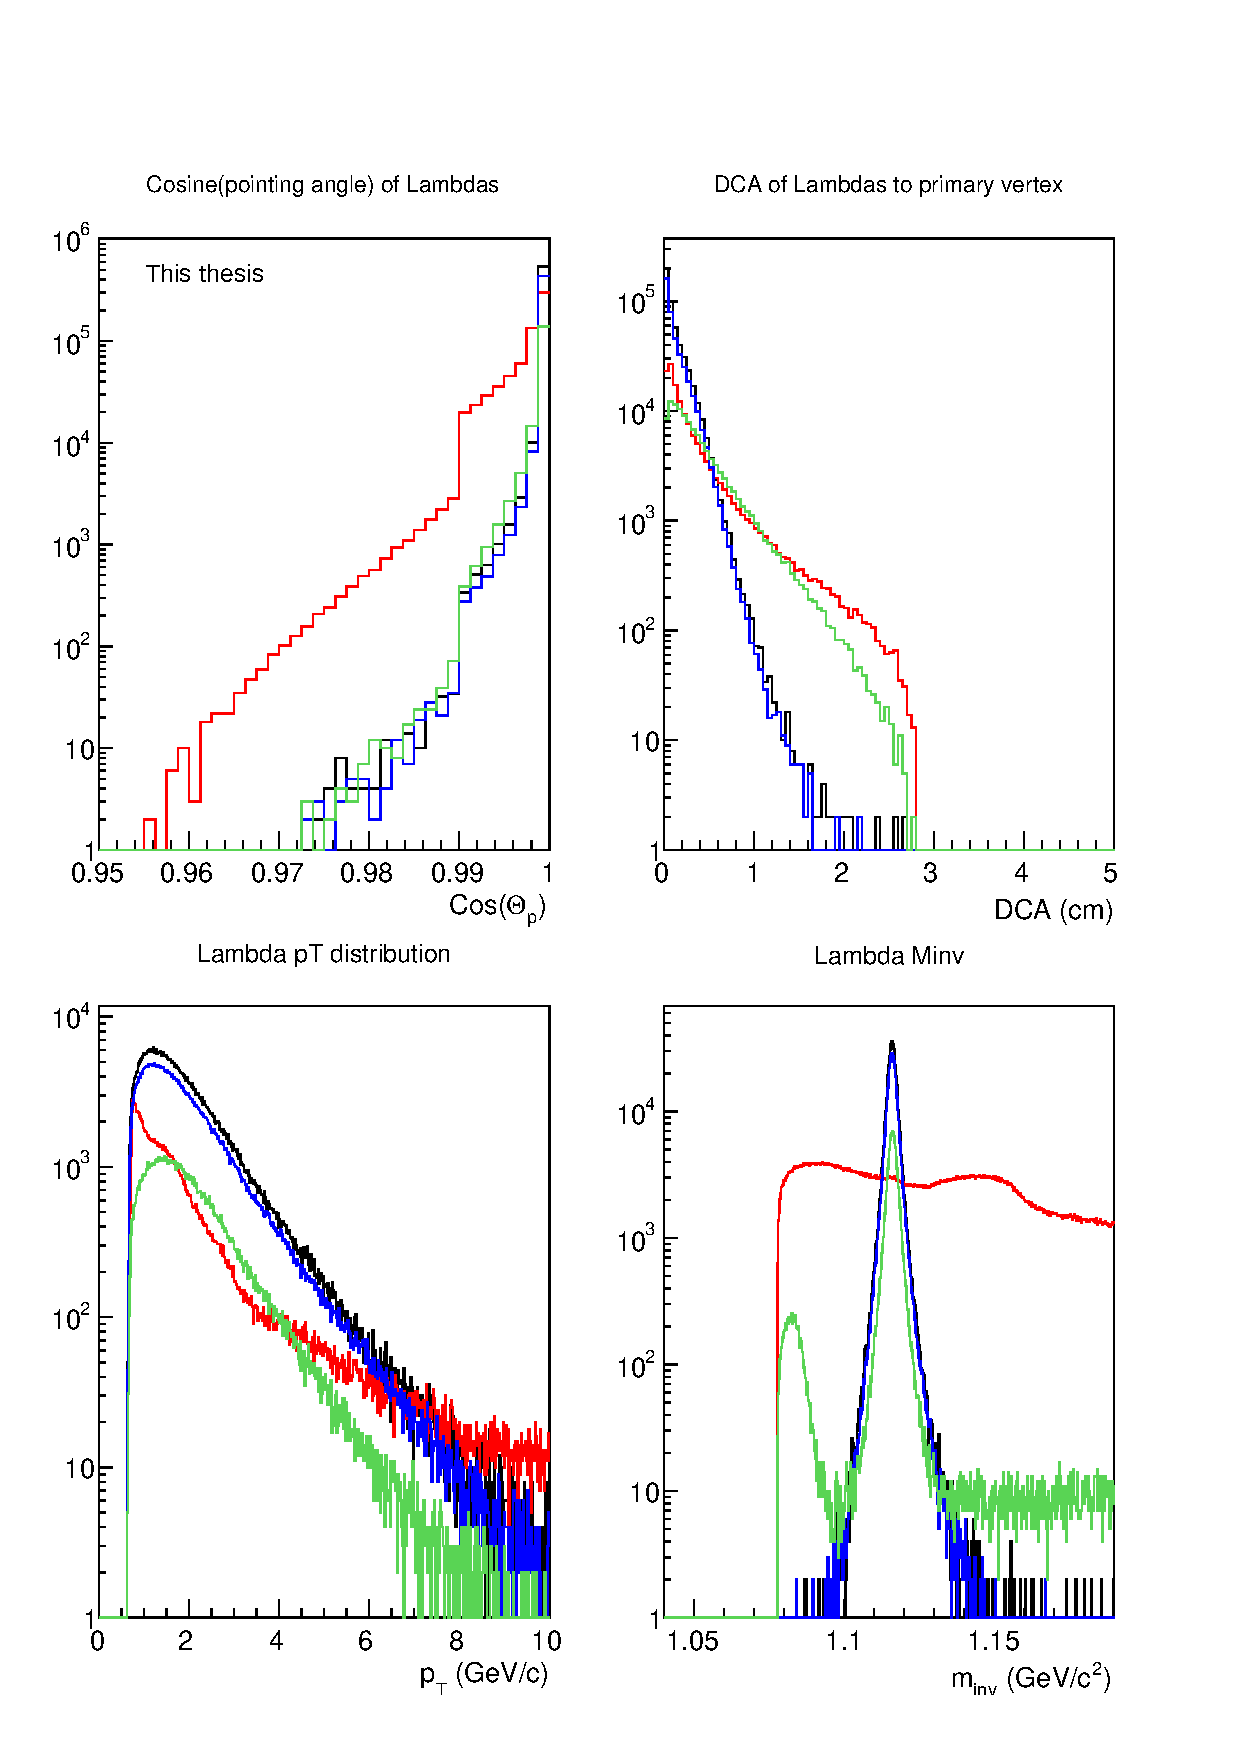
\includegraphics[width=36pc]{Figures/2014-03-31-Distribution-Lambda-4Types-CosP-DCA-pT-Minv.pdf}
\caption[$\Lambda$ cut distributions]{$\Lambda$ cut distributions shown for real $\Lambda$ (black), $\Lambda$ from $\Sigma$ decay (blue), secondary $\Lambda$ from other sources (green), fake $\Lambda$ (red). Optimal cut values were set such that a looser cut would differentially add more fake and (non-$\Sigma$) secondary $\Lambda$ than primary $\Lambda$}
\label{fig:LambdaCutDists1}
\end{figure}

\begin{figure}
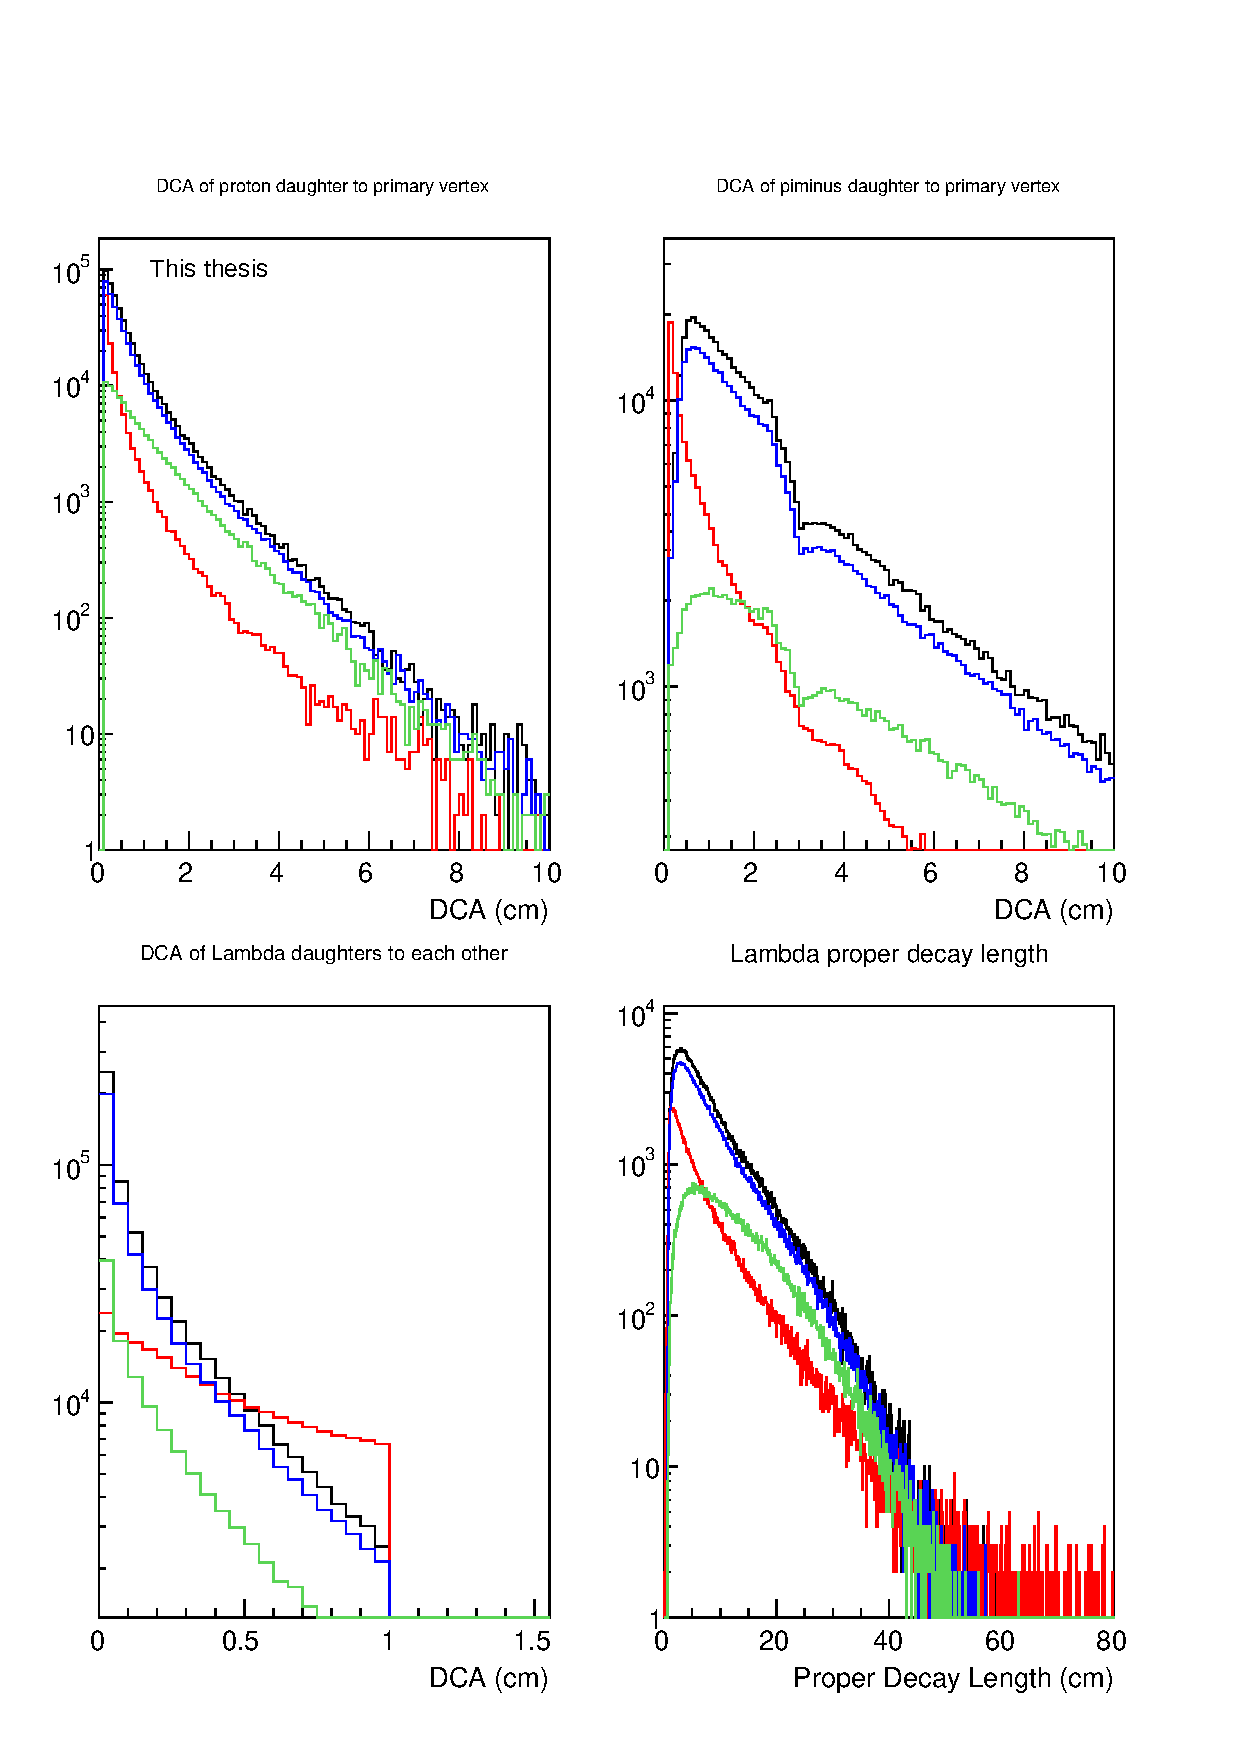
\includegraphics[width=36pc]{Figures/2014-03-31-Distribution-Lambda-4Types-DCA-DCA-DCA-DecayLength.pdf}
\caption[$\Lambda$ cut distributions]{$\Lambda$ cut distributions shown for real $\Lambda$ (black), $\Lambda$ from $\Sigma$ decay (blue), secondary $\Lambda$ from other sources (green), fake $\Lambda$ (red). Optimal cut values were set such that a looser cut would differentially add more fake and (non-$\Sigma$) secondary $\Lambda$ than primary $\Lambda$}
\label{fig:LambdaCutDists2}
\end{figure}

\begin{figure}
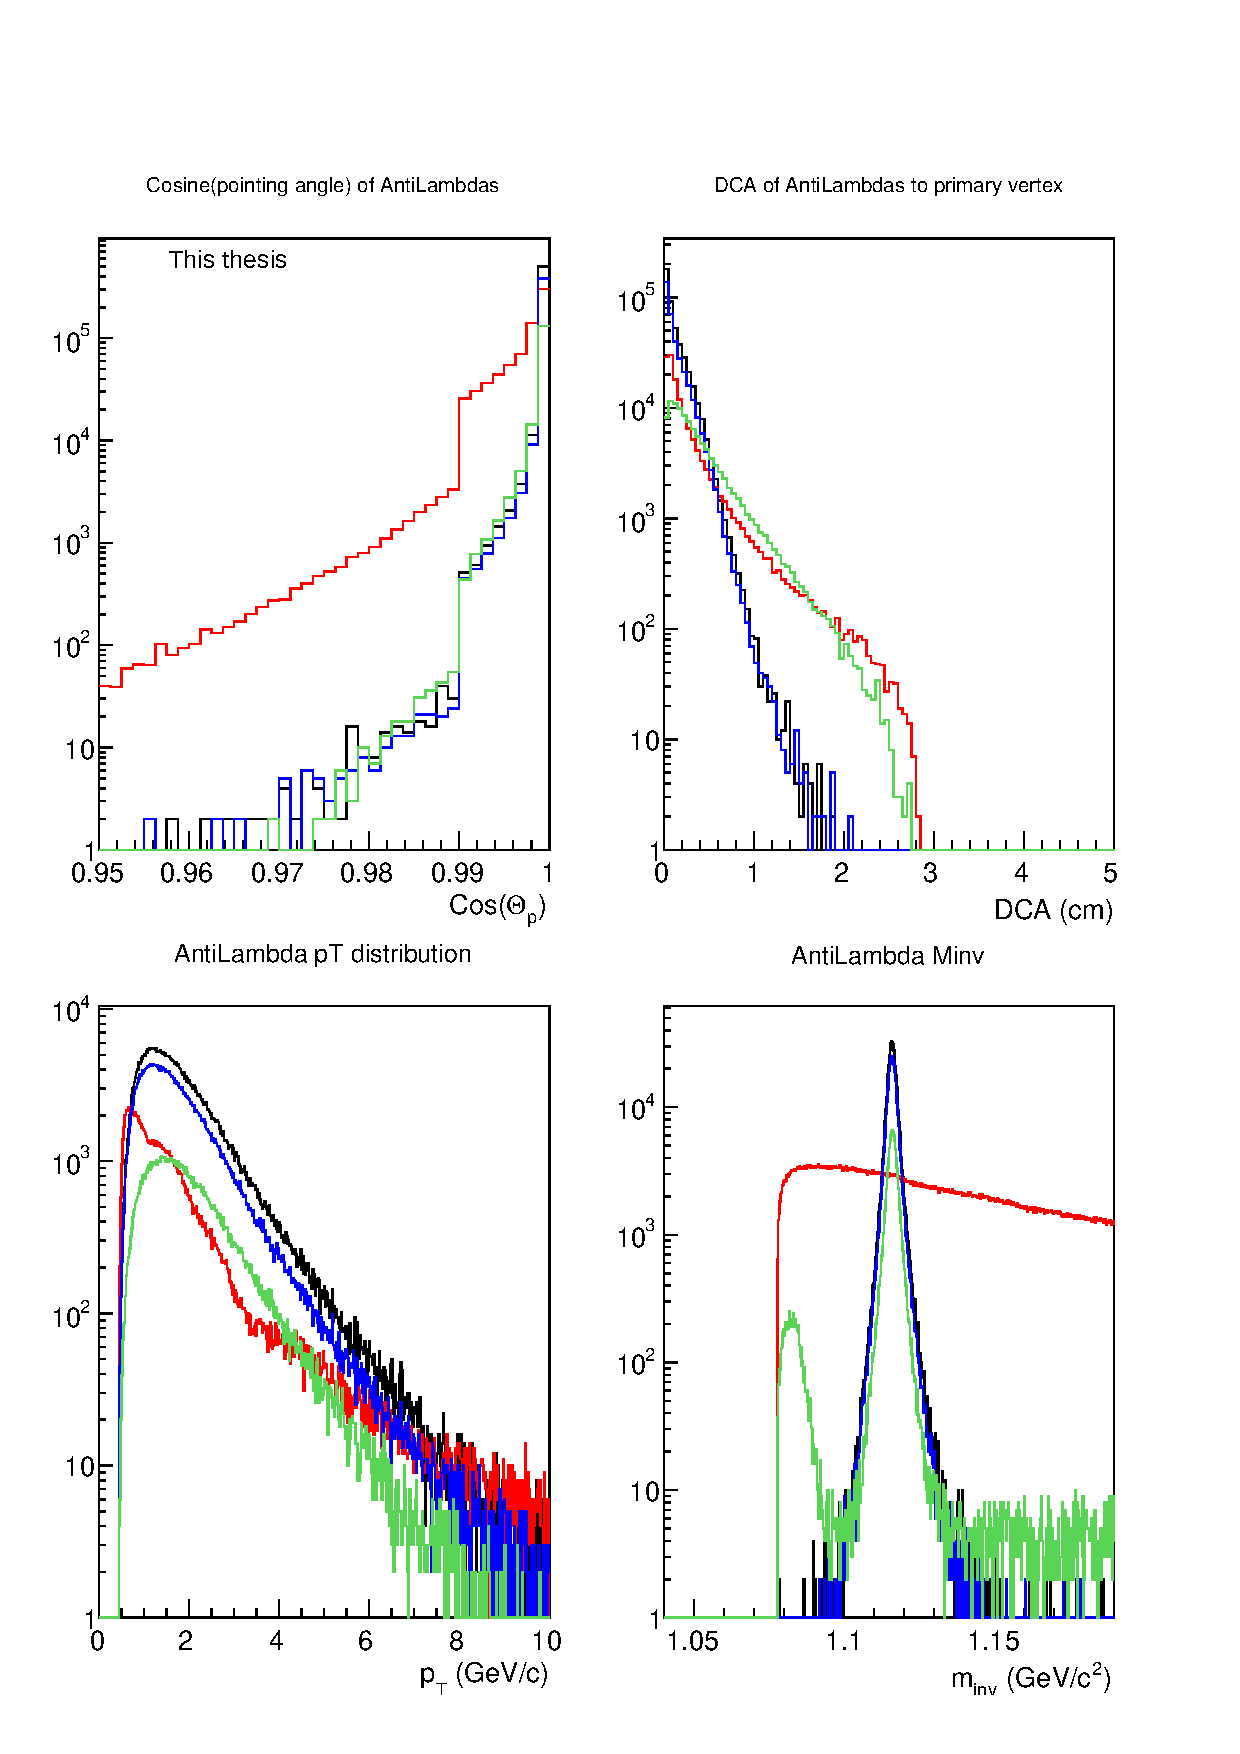
\includegraphics[width=36pc]{Figures/2014-03-31-Distribution-AntiLambda-4Types-CosP-DCA-pT-Minv.pdf}
\caption[$\bar{\Lambda}$ cut distributions]{$\bar{\Lambda}$ cut distributions shown for real $\bar{\Lambda}$ (black), $\bar{\Lambda}$ from $\Sigma$ decay (blue), secondary $\bar{\Lambda}$ from other sources (green), fake $\bar{\Lambda}$ (red). Optimal cut values were set such that a looser cut would differentially add more fake and (non-$\bar{\Sigma}$) secondary $\bar{\Lambda}$ than primary $\bar{\Lambda}$}
\label{fig:AntiLambdaCutDists1}
\end{figure}

\begin{figure}
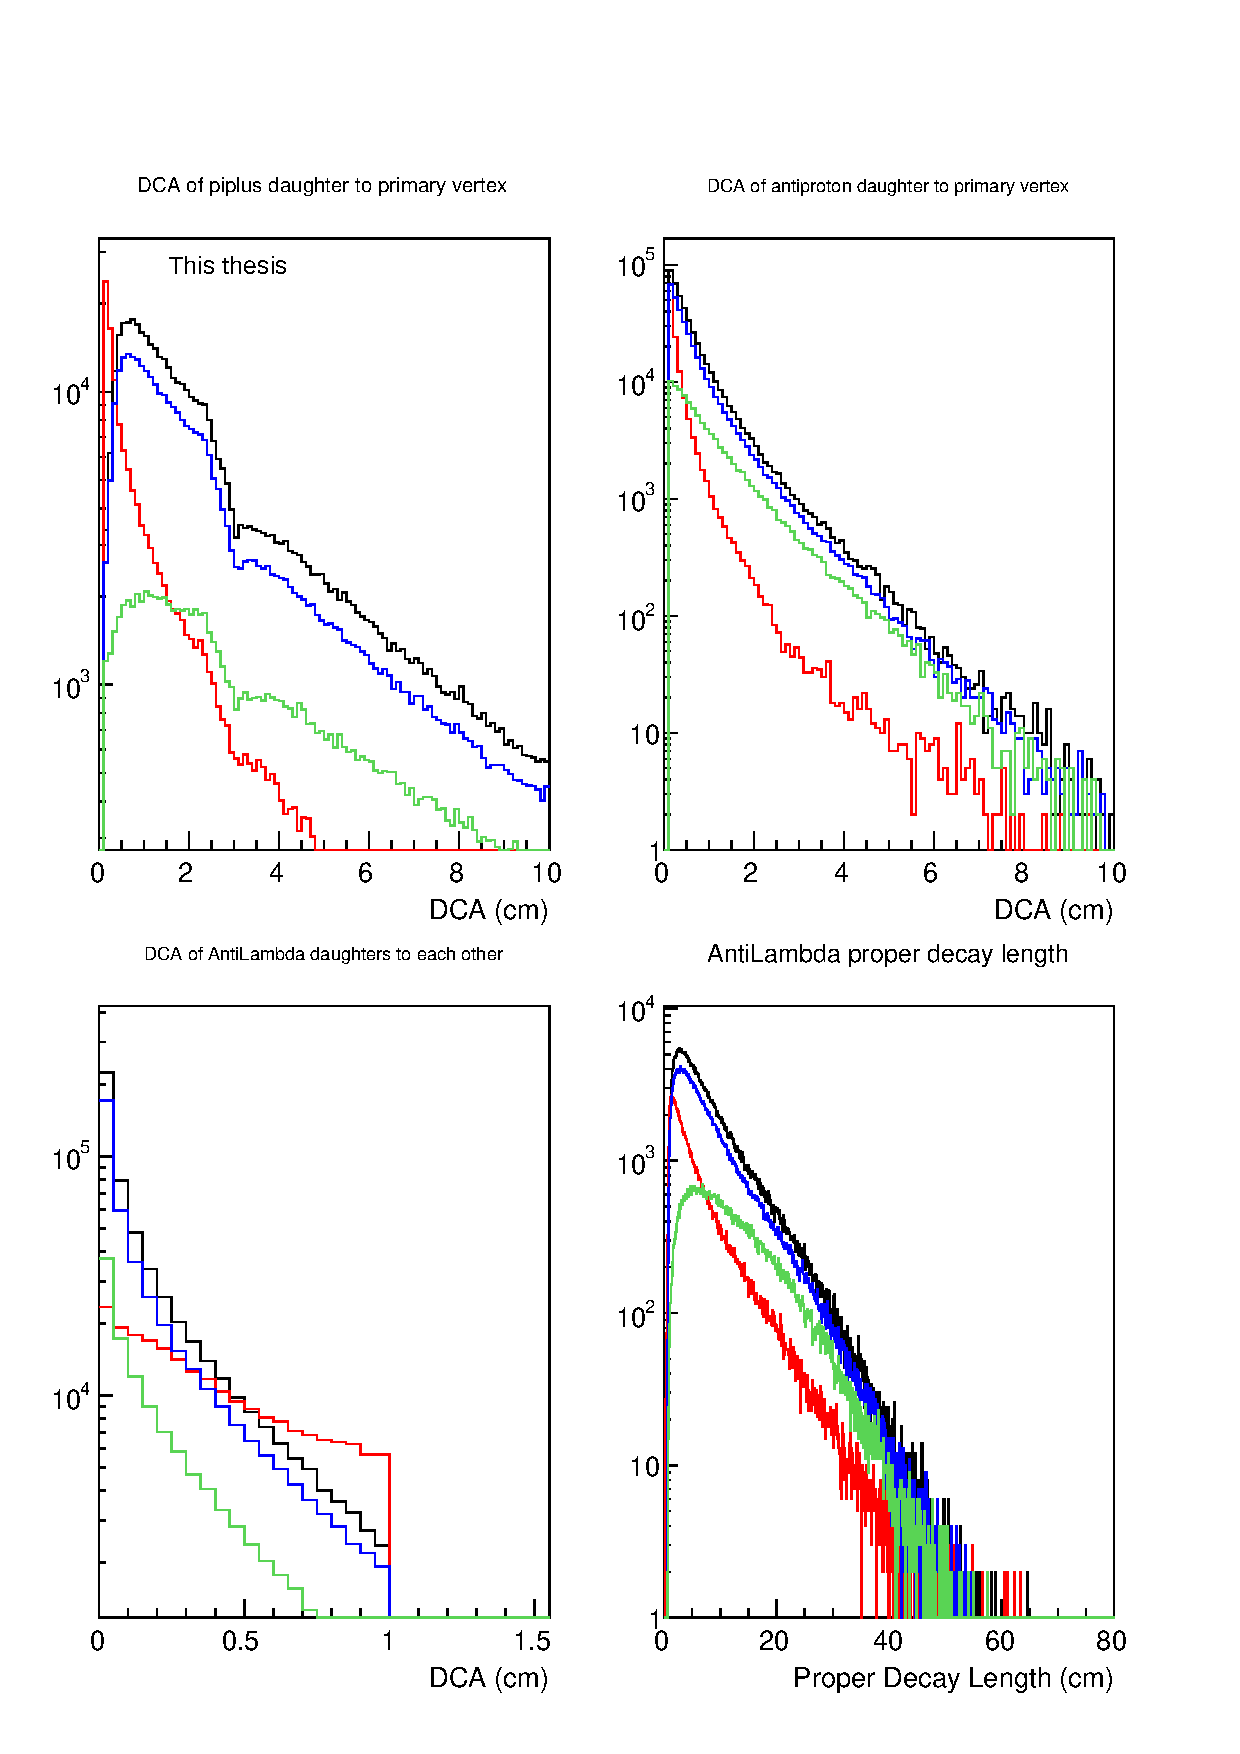
\includegraphics[width=36pc]{Figures/2014-03-31-Distribution-AntiLambda-4Types-DCA-DCA-DCA-DecayLength.pdf}
\caption[$\bar{\Lambda}$ cut distributions]{$\bar{\Lambda}$ cut distributions shown for real $\bar{\Lambda}$ (black), $\bar{\Lambda}$ from $\Sigma$ decay (blue), secondary $\bar{\Lambda}$ from other sources (green), fake $\bar{\Lambda}$ (red). Optimal cut values were set such that a looser cut would differentially add more fake and (non-$\bar{\Sigma}$) secondary $\bar{\Lambda}$ than primary $\bar{\Lambda}$}
\label{fig:AntiLambdaCutDists2}
\end{figure}

For the construction of Figures \ref{fig:LambdaCutDists1},\ref{fig:LambdaCutDists2},\ref{fig:AntiLambdaCutDists1}, and \ref{fig:AntiLambdaCutDists2}, each $\Lambda$ type was preselected using AliAODMCParticle information, and only V0 candidates of that type were reconstructed in that analysis run. This was done for ease of histogramming the distributions.  Roughly equal numbers events were analyzed for each run type, with the exception of the analysis of the primary $\Lambda$.  That analysis run utilized only about half the data set.  Therefore, the primary $\Lambda$ ($\bar{\Lambda}$) distributions in Figures \ref{fig:LambdaCutDists1},\ref{fig:LambdaCutDists2},\ref{fig:AntiLambdaCutDists1}, and \ref{fig:AntiLambdaCutDists2} have been scaled by a factor of 2 to compensate.

In these figures, both the shape and magnitude of each distribution is relevant for determining the cuts. For each cut type, a cut value was selected such that a looser cut would differentially accept more fake or secondary $\Lambda$ than primary $\Lambda$. Ideally, these cuts would be selected to reduce the inclusion of all types of secondary $\Lambda$.  However, it can be seen from the distributions that $\Lambda$ that come from $\Sigma$ decay display virtually the same cut parameter distribution shapes as primary $\Lambda$.  Only the magnitude of the $\Sigma$ curves differ from the primary $\Lambda$ curves.  This is due to the short decay length of the $\Sigma$ decay: $c\tau \approx 20$ pm for $\Sigma^0$ , and $c\tau \approx 6$ fm for $\Sigma$(1385). As a result, secondary $\Lambda$ from $\Sigma$ look identical to primary $\Lambda$, and they cannot be selectively removed from the analysis.

The systematic errors associated with these cut choices are discussed in Section \ref{sec:SystematicsReconstruction}. Further discussion of the reconstruction efficiency of the different $\Lambda$ types can be found in Section \ref{sec:ReconstructionEff}.

The reconstructed invariant mass distribution for $\Lambda$ and $\bar{\Lambda}$ can be seen in Figures \ref{fig:LamInvMass} and \ref{fig:ALamInvMass}. An approximation of the signal purity was estimated using a ratio of real and background (falsely reconstructed) counts.  The background was estimated using a fourth order polynomial.  The number of real $\Lambda$ was then estimated by counting the bin content and subtracting the background. The signal quality was found to be $real/(real + background) \approx 0.95$.  $\bar{\Lambda}$ were found to have approximately the purity.  From inspection of Figures \ref{fig:LamInvMass} and \ref{fig:ALamInvMass}, the $\bar{\Lambda}/\Lambda$ ratio is estimated to be about 93\%.

\begin{figure}[hbtp]
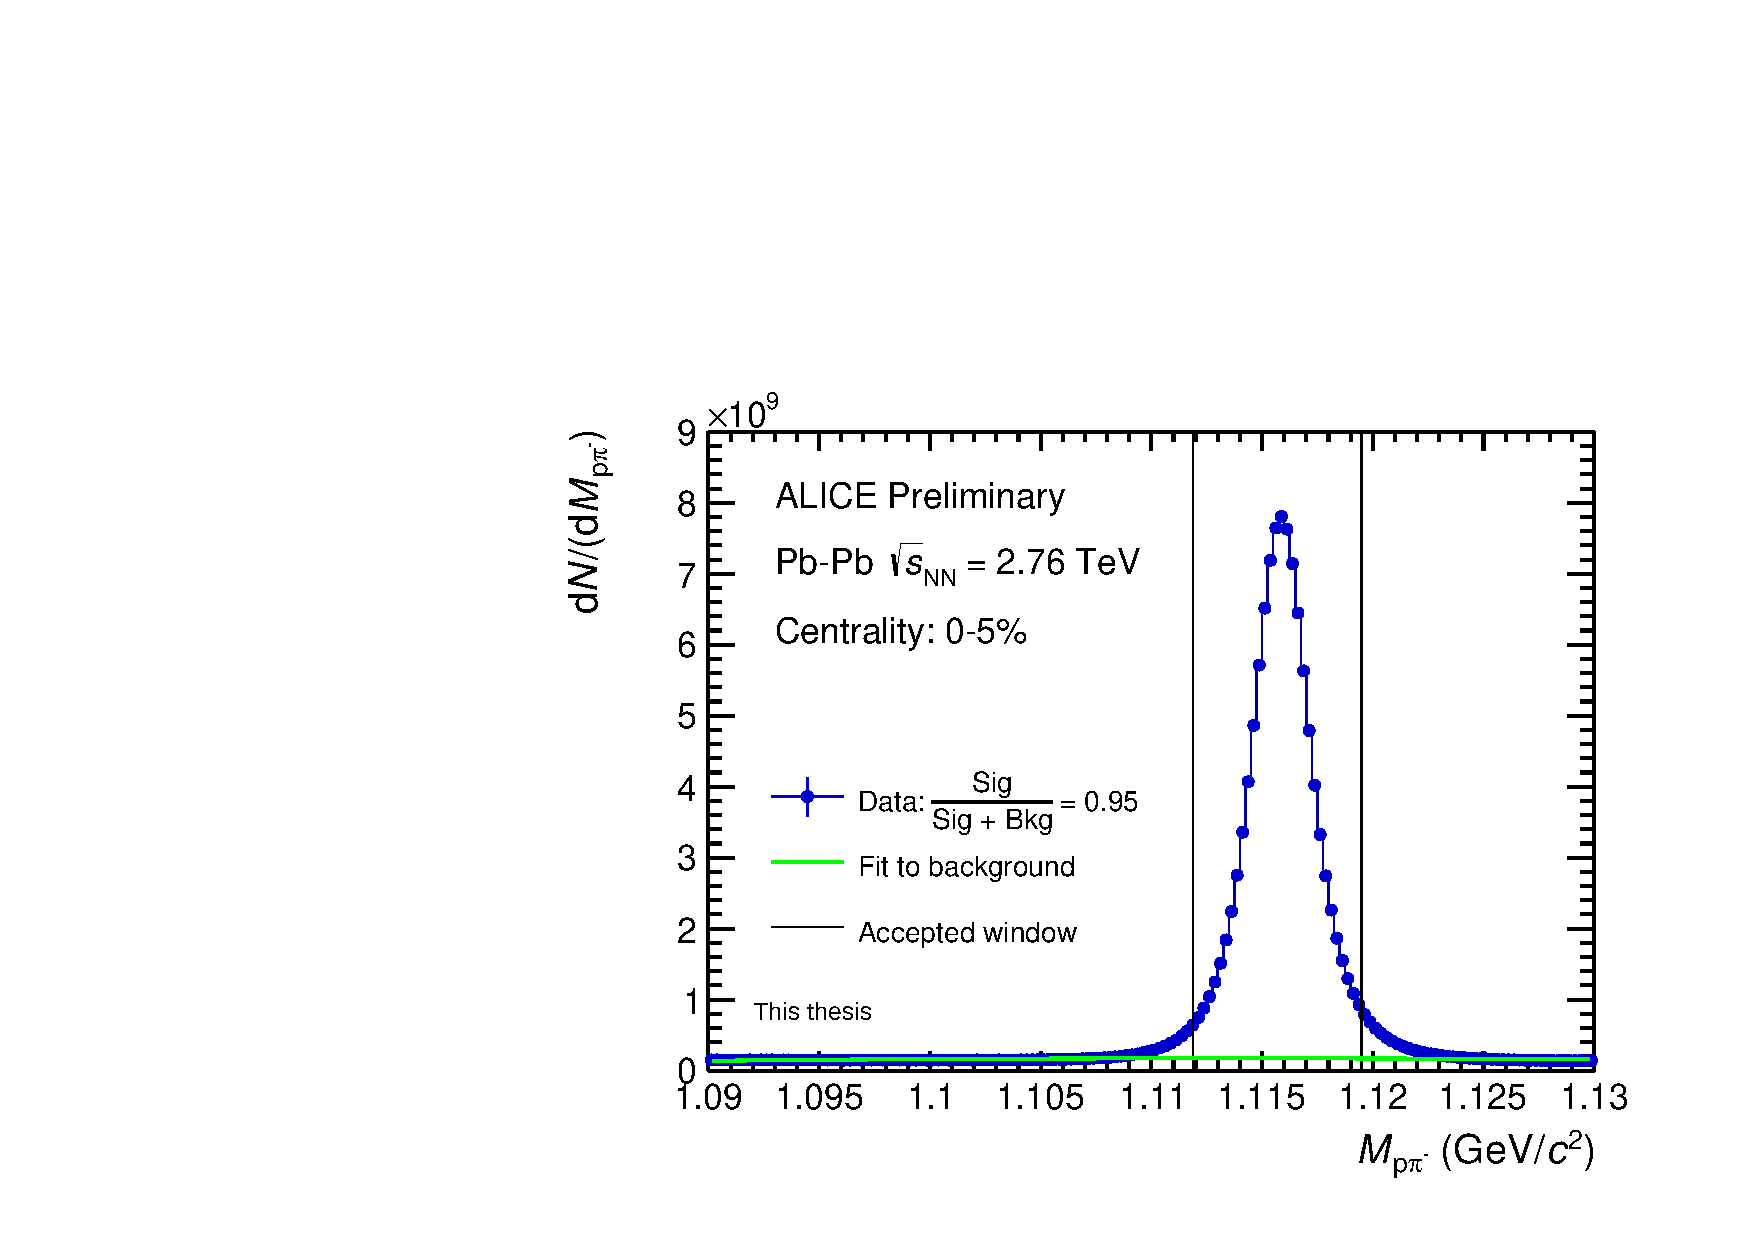
\includegraphics[width=36pc]{Figures/2014-05-11-LamMinv-CommentCorrections.pdf}
\caption[$\Lambda$ invariant mass distribution]{Invariant mass distribution for reconstructed $\Lambda$ using the optimal analysis cuts.  The plots show V0s reconstructed from centrality integrated LHC11h data.  The green line shows a fourth order polynomial fit to the background, which is used to estimate the number of real and fake $\Lambda$.  The estimated ratio of real $\Lambda$ to all reconstructed $\Lambda$ in the signal region ($ \lvert m_{\mathrm{inv}} - m_{\mathrm{PDG}}\rvert < 3.8$ MeV/$\rm c^2$) is approximately 0.95.}
\label{fig:LamInvMass}
\end{figure}

\begin{figure}[hbtp]
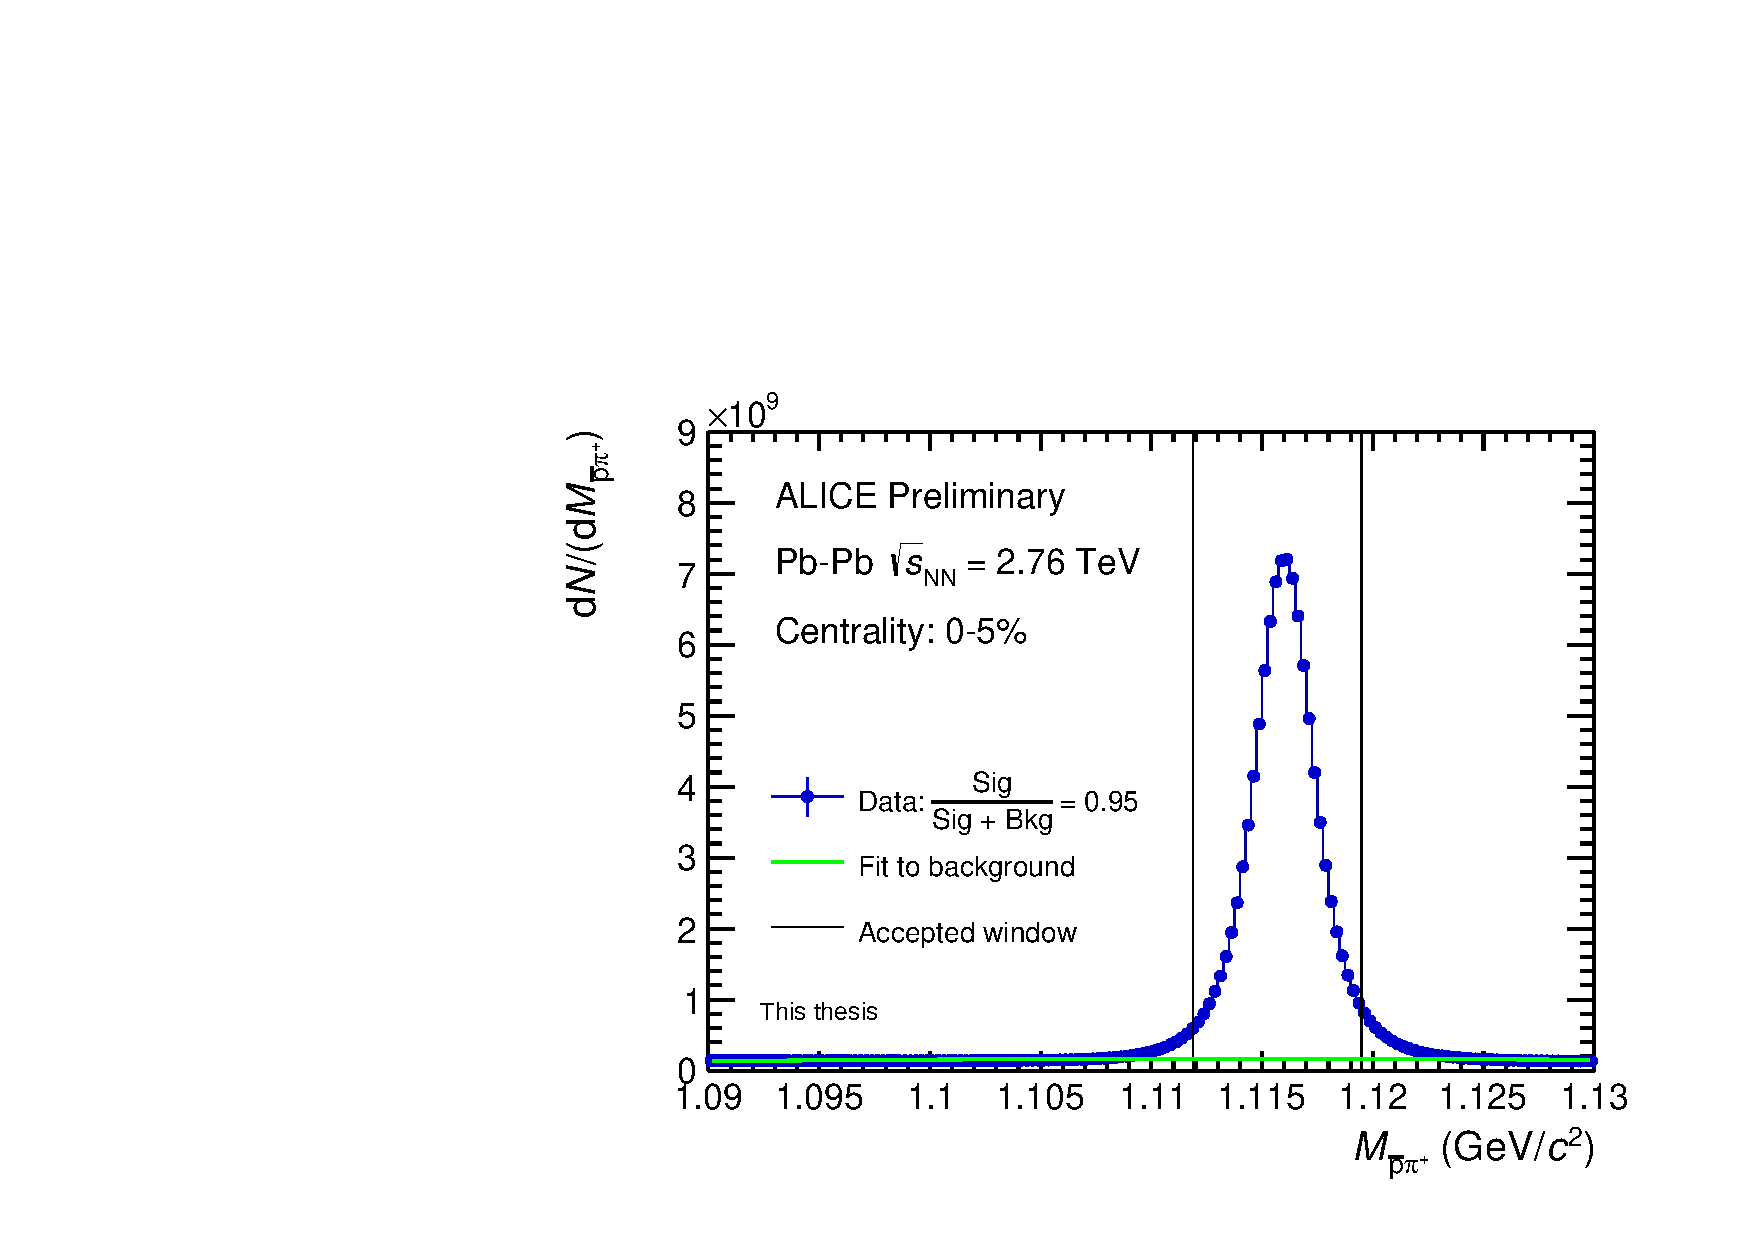
\includegraphics[width=36pc]{Figures/2014-05-11-ALamMinv-CommentCorrections.pdf}
\caption[$\bar{\Lambda}$ invariant mass distributions]{Invariant mass distribution for reconstructed $\bar{\Lambda}$ using the optimal analysis cuts.  The plots show V0s reconstructed from centrality integrated LHC11h data.  The green line shows a fourth order polynomial fit to the background, which is used to estimate the number of real and fake $\bar{\Lambda}$.  The estimated ratio of real $\bar{\Lambda}$ to all reconstructed $\bar{\Lambda}$ in the signal region ($ \lvert m_{\mathrm{inv}} - m_{\mathrm{PDG}}\rvert < 3.8$ MeV/$\rm c^2$) is approximately 0.95.}
\label{fig:ALamInvMass}
\end{figure}

\subsection{Decay radius (XY) cut}
The V0 finder includes a default decay radius cut of 0.9 cm, which removes V0s with a radial decay length less than that value.  This helps mitigate issues such as high track density which can complicate reconstruction.  This analysis currently only uses the default cut, though it is possible that a tighter cut could yield improved $\Lambda$ purity without severely impacting the available statistics.  The default cut will continue to be employed for now, but alternate cut values will be investigated in the future.  

Changes in this cut are expected to have only small effects on the correlation functions themselves.  As will be described later in this note, fits of correlation functions have a $\lambda$ parameter which accounts for the pair-purity (roughly the square of the single particle purity).  In any case, a few percent increase in purity should not drastically impact the shape of the correlation functions.


\subsection{Shared daughter cut}

Occasionally two or more V0s are reconstructed that both claim the same daughter track.  However, a given track can only be the daughter of, at most, one V0.  Therefore, if several reconstructed V0s all lay claim to the same daughter, at most only one of them can be a true V0.  It was decided to employ a cut that would compare characteristics of the different V0s to determine which of them was most likely to be the true parent particle.  After the best V0 was found, the competing V0s were removed from the list of V0 particles and not used during same- or mixed-event pair construction.

A study was done using MC event truths to determine which cut would be most successful at removing fraudulent V0s.  The following characteristics were examined as candidates for the cut criterion:

\begin{itemize}
\item Closeness of invariant mass to the PDG mass value.
\item DCA of the daughter particles to each other.
\item Cosine of the pointing angle.
\item DCA of the V0 to the primary vertex.
\end{itemize}

The process of culling V0s with shared-daughters was done by looping through V0s on an event-by-event basis after the V0 reconstruction process was completed.  For each V0 in the list of successfully reconstructed V0s (i.e. V0s that passed all cuts), the V0 was compared with each other V0 in the event to determine if they shared a daughter.  Two V0s "share" a daughter if both V0s have a charged daughter track with the same track ID.  When two V0s were found that shared a daughter, their values of the cut criterion were compared.  The daughter with the stricter value (e.g. smaller DCA to primary vertex) was adjudged to be the better V0 candidate, and the other V0 was flagged as "bad" for failing the shared-daughter cut.  V0s that failed the shared-daughter cut were not used in any pair construction (same event or mixed event).

However, it is possible for a V0 to share a daughter or daughters with two different V0s. In the aforementioned scheme, it is therefore possible for an excessive number of V0s to fail the shared daughter cut (excessive in that some of those failed V0s only shared a daughter with another failed V0).  To avoid throwing away too many V0s, a second loop was added to shared-daughter cut method to un-flag V0s that no longer share a daughter with any "good" V0. Example: V0s "A" and "B" both share a daughter, and V0s "A" and "C" share a different daughter.  "A" has a better DCA than "B", so "B" is flagged as bad.  Then "C" is found to have a better DCA than "A", so "A" is flagged as bad.  Finally, "B" is re-flagged as good because it no longer shares a daughter with any other good V0.

This method was adapted to run iteratively over the list of V0s candidates until a stable list of non-sharing V0s was found.  Then the MC truths of each V0 (those marked "good" and those marked "bad") were examined.  With this information, it is possible to calculate the percentages of true V0s and fake V0s that are removed via this process.  This analysis was run several times, each time using a different comparison criterion from the list above.

Based on the MC truth study, keeping the V0 with the closest DCA to the primary vertex was found to successfully keep 87\% of true V0s that had shared daughters.  In comparison, the cosine of pointing angle criteria was also successful 87\% of the time (cos$(\Theta_\mathrm{p})$ and DCA to primary vertex are strongly correlated), the DCA of daughters to each other criteria was successful 81\% of the time, and the absolute value of mass difference criteria was successful 79\% of the time.   Based on these results, the DCA to primary vertex criteria was selected to used for the shared-daughter cut before correlation function construction.

%On average there were two competing particles per every ... events in the MC study.  When applied to analysis of the LHC11h data, the rate was two per ....

One of the benefits of this cut is that it helps remove a splitting-like effect (see Section \ref{sec:PairWiseCuts} for more on splitting), wherein a true V0 shares each of its daughters with two separate fake V0s.  By the nature of the reconstruction cuts, all three of the V0s will be close in momentum space.  Therefore a pair constructed from the two fake V0s will contaminate the low relative-momentum region of the correlation function.  That pair of fake V0s does not share any daughters with each other, so it is not kept out of the correlation function by simple daughter ID checks.  But iterative daughter-sharing cut described above is capable removing this fraudulent pair, since either of the fake V0s is likely to be removed for sharing a daughter with the true V0.


\subsection{Correlation function construction and pair cuts}
\label{sec:CFconstruct}

This analysis studies two-particle correlations as a function of the one dimensional relative momentum $k^*=\frac{1}{2}q_{\mathrm{inv}}=\frac{1}{2}\abs{P(m^2_1-m^2_2)/P^2 - q}$, where $P$ and $q$ are the four-vector momentum sum and difference, respectively, and $m_1$ and $m_2$ are the masses of the two particles.  The correlation function is constructed as $C(k^*) = A(k^*)/B(k^*)$, where $A(k^*)$ is the two-particle distribution of the given event and $B(k^*)$ is the distribution of a reference event.  In practice, the signal event histogram $A(k^*)$ is constructed by binning the $k^*$ value of each pair of particles in a single event, and repeating this for each event.  The reference (or background) histogram is constructed by binning $k^*$ for pairs of particles taken from different events.  Care is taken to ensure that pairs are mixed from events with similar centralities (bin width of 5\%) and primary vertex z-position (2 cm bin width).  There are five mixed events for each real event.  When constructing pairs of V0s from the same event, the V0s are not allowed to share a daughter with the same track id. The correlation functions are normalized to unity in the $ 0.3 < k^* < 0.5$ GeV/c range.

\subsection{Pair-wise cuts}
\label{sec:PairWiseCuts}

Femtoscopic studies look at the relative momentum of particles, and often the most interesting physics lies at very low relative momentum (around 0.1 GeV/c and lower).  As a result, two-track reconstruction effects such as track splitting and track merging, both of which occur for tracks with similar momenta and trajectories, can have a large effect on the final results.  Track splitting means that the track left by a single charged particle is reconstructed as two separate tracks. Track merging is when the tracks of two separate particles are reconstructed as a single track.  For V0s, splitting/merging occurs on the level of the daughter tracks, and it affects the reconstruction of the parent V0s.

In this analysis, two-track reconstruction effects are combated via a cut on the average separation of daughter tracks from different lambdas.  The average separation distance of two daughter tracks are computed at nine different radii of the TPC.  The tracks are propagated iteratively using their local coordinates and the PropagateTo function, and their global positions are determined at 85, 105, 125, 145, 165, 185, 205, 225, and 245 cm.  Initial iteration is performed in 1 cm steps, though a secondary propagation is done in 0.1 cm steps for better precision.  Same- and mixed-event pairs are binned according to this separation distance.  To obtain an estimate of the merging/splitting effects both distributions are then scaled by the number of pairs at high average separation distance (10+ cm), and a correlation function (same event pairs/ mixed event pairs) is created. 

To ensure that average separation distributions of mixed-event pairs are comparable to the same-event distributions, it is necessary to perform a shifting of the primary vertex for mixed events.  Doing so allows the track separations to be calculated as though both events had the same primary vertex.  Without this correction, the mixed-event distributions are biased by differences in the primary vertex location.  One could imagine an extreme example of this if one used a 20 cm wide z-vertex bin.  In that case, tracks from different events could be shifted relative to each other by as much as 20 cm.  For this analysis with 2 cm z-vertex binning, and the uncorrected average separation correlation is shown in Figure \ref{fig:TwoTrackPerf} (left panel).  In contrast, the right panel of Figure \ref{fig:TwoTrackPerf} shows the primary-vertex corrected correlation.  To get a clear account of the difference between the two, we can look at Figure \ref{fig:TwoTrackRatio}, which shows the ratio of the corrected to uncorrected correlations.  The ratio is above unity from between 0 and 4cm.  We can interpret this to mean that the vertex-corrected distribution has more splitting and less merging than we would expect from the uncorrected plot.

Looking at Figure \ref{fig:TwoTrackPerf}, one can see that splitting effects are relevant out to about 1 cm, as evidenced by a relative abundance of same-event pairs.  Merging is visible out to about 3 cm, as evidenced by a dearth of same-event pairs in that range.  To address these effects, both same- and mixed-event V0 pairs are cut if they have a like-sign daughter pair with average separation less than 3 cm.  

However, one must be somewhat cautious here, since there are physics reasons to expect that $\Lambda\Lambda$ and $\Lambda\bar{\Lambda}$ should be suppressed at low relative momentum.  Some of that natural, physics-driven suppression may show up as a suppression in the average separation plots of the daughter tracks.  

One alternative/complement to using an average separation cut would be to enforce a relative decay length cut, where V0s are not paired with each other if their difference between their lab frame decay length values is less than some cut value (e.g. a few cm).  One advantage of this cut is that the decay lengths of the various particles should be independent of physics effects - i.e. independent of any quantum interference or final state interaction that might occur between the particles.  Meanwhile, the decay length cut may minimize daughter splitting effects, as well as some merging of low- and mid-$p_{\mathrm{T}}$ daughters.  High-$p_{\mathrm{T}}$ daughters may still be affected by merging, since higher-$p_{\mathrm{T}}$ particles have straighter trajectories in the TPC.  An analysis of relative decay length has not been performed yet, but it may prove a useful to combat splitting/merging effects.


%  In contrast, the average separation cut likely cuts out not only splitting/merging, but also some pairs with legitimate physics affects, since particles with low average separation are also close in relative momentum.  In the V0 case, neutral particles whose daughters are nearly collinear (i.e. small average separation) are themselves


%\begin{figure}[hbtp]
\begin{figure}[h]
\begin{minipage}{18pc}
%\includegraphics[scale=0.6]{Figures/2013-09-15-TwoTrackPerfUncorrected.pdf}
\includegraphics[width=18pc]{Figures/2013-09-15-TwoTrackPerfUncorrected.pdf}
\end{minipage}\hspace{2pc}
\begin{minipage}{18pc}
\includegraphics[width=18pc]{Figures/2013-09-15-TwoTrackPerfCorrected.pdf}
\end{minipage} 
\caption[Two-track reconstruction effects]{\label{fig:TwoTrackPerf}Correlation function versus average separation distance in the TPC for proton daughters.  Constructed using same-event pairs over uncorrected mixed-event pairs.  Both splitting (enhancement) and merging (suppression) effects are visible. The left panel shows the distribution with uncorrected mixed-event pairs, while the right panel shows the distributions with proper primary-vertex correction treatment.}
\end{figure}

\begin{figure}[hbtp]
\includegraphics[width=18pc]{Figures/2013-09-15-TwoTrackRatio.pdf}
\caption[Ratio of corrected/uncorrected average-separation distributions]{Ratio of vertex-corrected average separation plot to uncorrected average separation plot.  The enhancement above unity at low average-separation suggests that the uncorrected distribution underestimates the amount of splitting and overestimates the amount of merging.  The differences between the plots seems to disappear (i.e. ratio goes to unity at $\approx$ 3 cm.}
\label{fig:TwoTrackRatio}
\end{figure}

\subsection{Momentum resolution correction}
\label{sec:MomentumResCorrection}

There is an inherent resolution to V0 momenta that depends on the resolution of the reconstructed daughter tracks.  Because of this limit of precision, there is also an associated resolution to the relative momentum of two V0s.  The result of this resolution is that the reconstructed relative momentum of two V0s can be greater than or less than the true relative momentum of the two particles.  This momentum resolution effect can be treated as a roughly Gaussian smearing around a given $k^*$ value.  It introduces subtle changes to the measured correlation functions which must be corrected.

In this section, we will discuss the methodology used to make preliminary momentum resolution corrections.  This method captures the general features of the necessary correction, though more precise corrections and better (smaller) estimates of the associated systematic errors will be made at a later date.  The systematic errors coming from this study will be discussed in Section \ref{sec:MomentumResCorrectionsSys}.

The momentum resolution correction is a multiplicative correction factor in $k^*$ that is used to modify the various correlation functions:
\begin{equation}
C_\mathrm{corrected}(k^*) = C_{\mathrm{experimental}}(k^*)*F_\mathrm{correction}(k^*).
\end{equation}
The correction factor is constructed as a ratio of the true correlation function divided by the reconstructed correlation function
\begin{equation}
F_\mathrm{correction}(k^*)=\frac{C_\mathrm{true}(k^*)}{C_\mathrm{recon}(k^*)}.
\end{equation}
This correction necessitates an assumption about the natural form of the correlation function.  We use the analytic form described in Section \ref{sec:AnalyticModel}.  The true and reconstructed correlation functions are created using simulated pair relative momenta.  It was found that using $10^6$ simulated pairs, the correction factor histograms converged to a consistent shape without requiring excessive CPU time.  The correlation functions were constructed via
\begin{equation}
\label{eq:Ctrue}
C_{\mathrm{true}} = \frac{ N(k^*_{\mathrm{true}},W(C_{\Lambda\Lambda}(k^*_{\mathrm{true}})))}{N(k^*_{\mathrm{true}},1)}
\end{equation}
\begin{equation}
\label{eq:Crecon}
C_{\mathrm{recon}} = \frac{ N(k^*_{\mathrm{recon}},W(C_{\Lambda\Lambda}(k^*_{\mathrm{true}})))}{N(k^*_{\mathrm{recon}},1)},
\end{equation}
where the pairs $N(k^*_\mathrm{true})$ are generated to resemble the phase space (i.e denominator) distributions of the correlation function data -- roughly quadratic at low $k^*$ ($\lesssim 0.3 \ \mathrm{GeV}/c$).  The pairs $N(k^*_\mathrm{recon})$ are generated by taking each pair of $N(k^*_\mathrm{true})$ and adding to it a Gaussian correction factor to account for the momentum smearing.  The pairs are applied in the correlation function denominators with a weight of one.  They are applied in the numerator using as a weight the analytic form of the correlation function evaluated at that particular $k^*_{\mathrm{true}}$ value.  As such, $C_{\mathrm{true}}(k^*)$ resembles the assumed analytic form of the correlation function, while $C_{\mathrm{recon}}(k^*)$ shows how it looks with momentum smearing.  The correction $F(k^*)$ therefore is the factor that allows us to transform the experimentally constructed correlation functions to account for the momentum resolution effects.

\begin{figure}
\includegraphics[width=36pc]{Figures/2014-05-10-MomentumSmearingFitLL.pdf}
\caption[Relative momentum smearing]{Relative momentum smearing ($k_{\mathrm{smearing}} = k^*_{\mathrm{reconstructed}} - k^*_{\mathrm{truth}}$) for $\Lambda\Lambda$ pairs in MC events.  The extracted width of the distribution is approximately 10 MeV/c.}
\label{fig:MomSmearingFit}
\end{figure}

To obtain the width of the momentum smearing, a MC analysis is performed in which $k*_{\mathrm{smeared}} = k^*_{\mathrm{reconstructed}} - k^*_{\mathrm{truth}}$ is binned.  $k^*_{\mathrm{truth}}$ is determined from looking at the associated AliAODMCParticles of the reconstructed tracks.  The analysis is only performed for real V0s.  Fake V0s (as defined in Section \ref{sec:Recon}) were omitted, as they have no true momenta.  The analysis did not distinguish between primary and secondary $\Lambda$, as both are affected by momentum resolution effects and both appear in the data.  The binning was done performed only for mixed-event pairs, as those pairs will reflect the momentum resolution effects on the overall phase space without including any complications from physics interactions.  At this time, the binning was done in a centrality integrated fashion -- future studies could look to see if and how the effects differ between centralities.  After obtaining this distribution for each pair type ($\Lambda\Lambda$, $\bar{\Lambda}\bar{\Lambda}$, and $\Lambda\bar{\Lambda}$), the each distribution was fit with a Gaussian in order to extract a characteristic width of the momentum smearing.  One such fit can be seen in Figure \ref{fig:MomSmearingFit}.  The large $\chi^2 /\mathrm{ndf}$ indicates that the smearing isn't well described by a Gaussian.  Part of that may be due to the $p_\mathrm{T}$ and centrality integrated nature of the histogram.  Nonetheless, a Gaussian width has been extracted that roughly characterizes the width of the smearing.  Each pair type returned a width that was within a couple percent of $10\ \mathrm{MeV}/c$.

As stated above, when constructing $C_\mathrm{true}$ and $C_\mathrm{recon}$, we used an analytic form of the correlation functions.  While the form is well specified (see Section \ref{sec:AnalyticModel}), it was necessary to assume values for the various parameters of the equation: radius, pair fraction ($\lambda$), scattering lengths, effective range of interaction.  Typically, thorough evaluations of the resolution correct use an iterative procedure as part of the process of fitting the correlation functions.  Values are assumed for the parameters, resolution corrections are made, and fits to the data are performed.  Then the process repeats.  As the current analysis is not yet at the stage of fitting, we've settled on a "best guess" for the values used here: radius $=2.5$ fm; $\lambda = 0.3$; real part of scattering length $= -0.5$ fm; imaginary part of scattering length $= 0$ fm for $\Lambda\Lambda$ and $\bar{\Lambda}\bar{\Lambda}$, and $0.5$ fm for $\Lambda\bar{\Lambda}$; and the effective range $=3$ fm.  These numbers were chosen agnostic of the centralities being fit, where very early fit attempts have estimated radii between 2.7 fm and 2.3 fm.  

Figures \ref{fig:MomCorrectionFactorLLAA} and \ref{fig:MomCorrectionFactorLA} show the momentum resolution correction histograms for $\Lambda\Lambda$/$\bar{\Lambda}\bar{\Lambda}$ and $\Lambda\bar{\Lambda}$ respectively.  The dip in the correction factor at low $k^*$ shows that the effect of the momentum resolution on the reconstructed correlation function is to flatten (i.e. raise towards unity) the correlation function in that region).  The correction factor serves to undo that flattening.  At its largest it is about a three percent correction for $\Lambda\Lambda$/$\bar{\Lambda}\bar{\Lambda}$.  The effect is wider but also shallower for $\Lambda\bar{\Lambda}$, where at its max it is less than a one percent correction.  In this preliminary momentum resolution correction, the same resolution correction will be applied to each centrality range for a given pair type.  

\begin{figure}
\includegraphics[width=36pc]{Figures/2014-05-10-PrelimCorrectionFactorLLAA.pdf}
\caption[Relative momentum correction factor for $\Lambda\Lambda$ and $\bar{\Lambda}\bar{\Lambda}$]{A histogram of the relative momentum correction factors used to correct $\Lambda\Lambda$ and $\bar{\Lambda}\bar{\Lambda}$ correlation functions.  The corrected correlation function is found by multiplying each $k^*$ bin of the experimentally measured correlation function by the associated bin of the correction factor.  The dip in the correction factor at low $k^*$ shows that the effect of the momentum resolution on the reconstructed correlation function is to flatten (i.e. raise towards unity) the correlation function in that region).  The correction factor serves to undo that flattening.  At most it is about a three percent correction.}
\label{fig:MomCorrectionFactorLLAA}
\end{figure}

\begin{figure}
\includegraphics[width=36pc]{Figures/2014-05-10-PrelimCorrectionFactorLA.pdf}
\caption[Relative momentum correction factor for $\Lambda\bar{\Lambda}$]{A histogram of the relative momentum correction factors used to correct $\Lambda\bar{\Lambda}$ correlation functions.  The corrected correlation function is found by multiplying each $k^*$ bin of the experimentally measured correlation function by the associated bin of the correction factor.  Except for the lowest bin, the dip in the correction factor at low $k^*$ shows that the effect of the momentum resolution on the reconstructed correlation function is to flatten (i.e. raise towards unity) the correlation function in that region).  The correction factor serves to undo that flattening.  The effect is seen to be less than a one percent correction}
\label{fig:MomCorrectionFactorLA}
\end{figure}

Because all the centralities are receiving the same multiplicative (and therefore commutative) correction, the shape of the final, centrality-merged, momentum-corrected correlation functions will be the same whether the correction is applied to each 5\% centrality bin or to the merged correlation functions.  For the purpose of determining systematic uncertainties, the correction will be done on the merged correlation functions.  The size and shape of the momentum smearing is highly dependent on the analytic form of the correlation function, and it is therefore dependent on the chosen values of the parameters.  This sensitivity, along with the currently centrality-independent nature of the correction, will be accounted for in the systematic uncertainties by applying a conservative (i.e. large) uncertainty for this effect.  

\section{Systematic errors}
\label{sec:GeneralCfSysErrorDiscussion}

We will now attempt to identify the various systematic effects that may affect the correlation functions.  The goal will be to quantify the systematic uncertainties associated with each $k^*$ bin.  It should be noted, however, that subsequent fits to the correlation functions are not directly impacted by these error bars.  Instead, the systematics on the resulting fit parameters will be computed by refitting many versions of the correlation functions (e.g. those built with different reconstruction cuts) and comparing the results. This will be discussed in greater detail in Section \ref{sec:FitSystematics}.

\subsection{Consistency checks for uncorrelated histograms}
\label{sec:ConsistencyCheckUncorrelated}
One of the tools we will employ in the search for systematic effects is the TH1::Chi2Test(TH1* h1) method, which compares two histograms bin-by-bin to determine a $\chi^2$.  The test is performed assuming the hypothesis that the two histograms are Poissonian samples of the same underlying distribution.  A p-value is computed which represents the probability that a measurement could be performed that would yield results this different or more, given the hypothesis of identity.  The hypothesis of identity is rejected in instances where the p-value is lower than 0.01. At that threshold, less than one percent of tests will fail of data sets sampled from the same underlying distribution.  This corresponds to rejecting the hypothesis of identity for data samples that differ by roughly $3 \sigma$.  The 0.01 metric is somewhat arbitrary - it was chosen to be small enough that pure statistical fluctuations should not often lead to false or unnecessary systematic errors.  For example, if a p-value of 0.1 were used instead, this would result in roughly 10\% of "good" results failing the test and contributing to the uncertainty, which would lead to a gross overestimation of the total systematic error.  Similarly, a threshold of 0.001 would probably underestimate the error.  Thus, 0.01 was chosen.

In this analysis, Chi2Test() will be used to compare two correlation functions which are uncorrelated with each other (uncorrelated in the sense that they are completed independent data samples).  One example where this can be employed is the comparison of correlation functions constructed using data taken under different field configurations.  This analysis needs all the data available to it, so results taken under different field configurations will need to be merged to improve statistics.  But before they are combined, it must be checked that they contain compatible results.  The Chi2Test() method provides a means of characterizing the degree of similarity of the correlation functions.  

Correlation functions that surpass the significance level of 0.01 will be treated as being functionally the same within statistics, and their weighted average will be computed without recourse to systematic uncertainty. In the instances where they do not exceed the significance level, they will be analyzed on a case-by-case basis.  In particular, we will look to see if there are any systematic differences between the correlation functions.  For example, it may be seen that the lowest ten $k^*$ bins will all be higher in one correlation function than another.  If so, the data will still be merged (so long as the results aren't dramatically different), but a systematic uncertainty will be computed and applied to the final averaged correlation function in the form of systematic error bars.  Section \ref{sec:CalculatingSysErrors} describes how these uncertainties are calculated.  

When using Chi2Test() to compare correlation functions, the trouble areas that result in small p-values will likely be the lowest $k^*$ bins (which exhibit most of the interesting physics, and which also suffer the most from two-track effects), and large $k^*$ bins (close to $1 \mathrm{GeV/c}$).  The height of the the large $k^*$ bins is noticeably susceptible to statistical (or systematic) deviations in the normalization region.  The high $k^*$ bins have relatively small statistical error bars, so small deviations of normalization between correlation functions can result in large $\chi^2$ values.  The correlation functions are all normalized to unity in the $0.3 < k^* < 0.5 \mathrm{GeV}/c$ range, so there are unlikely to be significant deviations seen in that range.  

It is important to emphasize that Chi2Test() is only appropriate for comparing two uncorrelated histograms.  In the case of correlated histograms (e.g. correlation functions constructed using slightly different two-track cuts or different reconstruction cuts), a different method must be used to test the histograms for consistency.  


\subsection{Consistency checks for correlated histograms}
\label{sec:ConsistencyCheckCorrelated}
Chi2Test() cannot be used to compare correlated data because the test is performed assuming the statistical error bars on the two histograms are independent.  That is obviously not the case for two histograms that differ in their data only be a few percent.  In this analysis, we perform consistency checks of correlated data in the following fashion:

\begin{enumerate}
\item Take the difference between the two correlation function histograms $\Delta C(k^*) = C_1(k^*) - C_2(k^*)$, using $C_1\rightarrow$ Add($C_2$,$-1$).  The resulting histogram shows the usually small differences between the two data sets.
\item Here, ROOT incorrectly adds the errors in quadrature.  To fix this, manually set the error bars using $\sigma_{\Delta}(k^*) = \sqrt{ \abs{ \sigma_1^2(k^*) - \sigma_2^2(k^*) }}$.  This error is correct in the specific case (found here) that one histogram is entirely a subdivision of the other.
\item If there are no significant discrepancies or systematic differences between the two original correlation functions, the difference histogram should be consistent with zero.  We can test this using TH1::Chisquare(TF1*), and fit the data with the function $y=0$.  Chisquare() returns the $\chi^2$ value of the fit.
\item We acquire a p-value for this consistency check using TMath::Prob(Double chi2, int ndf), which takes as input the $\chi^2$ from the fit and the number of $k^*$ bins as the number of degrees of freedom.  
\item Finally, we evaluate the two correlation functions as either consistent or inconsistent depending on if they pass or fail the p-value test.  A p-value $\geq 0.01$ passes.  
\item All pairs of histograms with p-values below that threshold are considered to have significant differences.  All such pairs are considered to introduce a $k^*$-dependent systematic error for the correlation function measurement in that particular centrality bin.  The method for evaluating the size of that systematic error is described in the following section.
\end{enumerate}

Using the steps listed above, we can evaluate if subtle changes to the cuts employed in correlation function construction change the resulting data in any significant way.  

%The study of normalized residuals (the difference between the bin contents and the expected bin contents) can be used to characterize which regions are responsible for small p-values.  This is again handled by the Chi2Test() method.  For each $k^*$ bin, a normalized residual plot shows the number of $\sigma$ differences between the two correlation functions.  This can make it easy to look for systematic differences, even in the case of small shifts at high $k^*$, which would be hard to see by eye in the raw correlation functions.

\subsection{Calculating systematic errors for data sets that fail p-value tests}
\label{sec:CalculatingSysErrors}

The general scheme for calculating systematic uncertainties is to take the difference between two correlation functions (which have failed a p-value test), and then fit that difference with a polynomial.  For each $k^*$ bin, the absolute value of the fit polynomial evaluated at the center of that bin is taken as the error for that bin.  The specifics of the procedure will be described in more detail below.

This procedure of using fits to extract systematic error is intended to produce representatively large systematic errors when there are systematic differences between the correlation functions.  It is further intended to produce small systematic errors when the (large or small) differences between the correlation functions are essentially statistical fluctuations.  For example, $\Delta C(k^*)$ exhibits a clear, systematic upward shift in a particular $k^*$ range, the fit will be pulled upward in that region.  In contrast, if $\Delta C(k^*)$ has large deviations away from zero, but those deviations are distributed roughly randomly above and below zero, then the fit should be small in magnitude (and therefore give a small systematic error).   

Initial attempts to use this fit method resulted in systematic error bars that grew in size with the statistical error bars.  That is, the measured systematic and statistical errors seemed strongly correlated.  To reduce the statistical dependence of the fitting procedure, the correlation functions were rebinned to have fewer bins (and more statistics in each bin) before fitting.

Both uncorrelated data (Sec.\ \ref{sec:ConsistencyCheckUncorrelated}) and correlated data (Sec.\ \ref{sec:ConsistencyCheckCorrelated}) are fit in essentially the same way.  In both instances, the relevant correlation functions are reconstructed using rebinned numerators and denominators via TH1::Rebin(int).  Rebin(4) reduces the number of bins in the correlation functions by a factor of four.  The resulting rebinned correlation functions maintain the same general features and shape of the original correlation functions, but statistical fluctuations are significantly damped down. This was found to generally reduce the size of the error fit function, compared with fitting un-rebinned data.  

The difference of the two rebinned correlation functions is calculated as $\Delta C_{\mathrm{rebin}}(k^*) = C_{1,\mathrm{rebin}}(k^*) - C_{2,\mathrm{rebin}}(k^*)$.  For correlated data, the statistical uncertainties of $\Delta C(k^*)$ are calculated as described in Section \ref{sec:ConsistencyCheckCorrelated}.  Otherwise, ROOT correctly handles the statistical uncertainties for uncorrelated data.

$\Delta C_{\mathrm{rebin}}(k^*)$ is then fit with a fifth order polynomial.  The polynomial is converted into a histogram with the same number of $k^*$ bins as the original, un-rebinned correlation functions.  Finally, the contents of each bin is set to its absolute value.  The values of this histogram are taken to be the symmetric systematic errors associated with the particular failed correlation function consistency check.

The sections below will discuss the specific details of looking for and evaluated systematic errors associated with different magnetic field configurations of the detector, different V0 reconstruction cuts, and different two-track cuts. Section \ref{sec:CombiningSys} will discuss how the different sources of systematic error are combined and applied to the final correlation functions.

\subsection{Systematic errors associated with different run field configurations}
\label{sec:SystematicsFieldConfig}

In this section we discuss the systematic errors associated with the different field configurations ($++$ and $--$, see Section \ref{sec:DataSelection}).  Correlation functions are constructed separately for each pair type ($\Lambda\Lambda$, $\bar{\Lambda}\bar{\Lambda}$, and $\Lambda\bar{\Lambda}$), each 5\% centrality bin, and each field configuration.  For each centrality bin and pair type, we look for any non-statistical deviations in the correlation functions of the two field configurations via the application of Chi2Test().  Table \ref{tab:FieldPvalues} shows p-value results obtained from comparing the two different field results with Chi2Test().  For each pair type, most of the centrality bins pass the test - i.e. the correlation functions made with each field appear to sample from the same underlying distribution.  The few that do not pass have been analyzed using the fit method described in Section \ref{sec:CalculatingSysErrors} in order to quantify the systematic errors associated with their differences.  %Figure \ref{fig:ExampleFieldFailureSysErrors} shows the example results fitting the ... bin for systematic errors.

\begin{table}
\begin{center}
\begin{tabular}{| c | c | c |}
  \hline                       
  Pair Type & Centrality Range & p-value \\
  \hline
  $\Lambda\Lambda$ & 0-5\% & .95  \\
   & 5-10\%  & .38 \\
   & 10-15\% & 3.4e-05 \\
   & 15-20\% & .71 \\
   & 20-25\% & .43 \\
   & 25-30\% & .62 \\
   & 30-35\% & .59 \\
   & 35-40\% & .06 \\
   & 40-45\% & .61 \\
   & 45-50\% & .31 \\
   \hline
  $\bar{\Lambda}\bar{\Lambda}$ &  0-5\% & .24 \\
   & 5-10\% & .03 \\
   & 10-15\% & .04 \\
   & 15-20\% & .02 \\
   & 20-25\% & .003 \\
   & 25-30\% & .87 \\
   & 30-35\% & .001 \\
   & 35-40\% & .02 \\
   & 40-45\% & .15 \\
   & 45-50\% & .31 \\
   \hline
  $\Lambda\bar{\Lambda}$ &  0-5\% & .87 \\
   & 5-10\% & .10 \\
   & 10-15\% & .25 \\
   & 15-20\% & 4.1e-05 \\
   & 20-25\% & .04 \\
   & 25-30\% & .11 \\
   & 30-35\% & .44 \\
   & 35-40\% & .03 \\
   & 40-45\% & .26 \\
   & 45-50\% & .011 \\
  \hline  
\end{tabular}
\label{tab:FieldPvalues}
\caption{p-values and $\chi^2$ calculated using the TH1::Chi2Test() method for correlation functions of different field configurations.  For a given pair type and centrality bin, correlation functions, with a p-value $\geq 0.01$ are assumed to sample the same underlying distribution.  For each pair type, one or two centralities are seen to fail the p-value test.  The differences between those centrality bins have been evaluated and the systematic errors associated with those differences have been quantified.}
\end{center}
\end{table}



%\begin{figure}
%\includegraphics[width=36pc]{Figures/***.pdf}
%\caption[]{}
%\label{fig:ExampleFieldFailureSysErrors}
%\end{figure}



\subsection{Systematic errors from reconstruction cuts}
\label{sec:SystematicsReconstruction}

In this section we discuss the systematic errors associated with the V0 reconstruction cuts (e.g. cosine of pointing angle, DCA to primary vertex, etc.).  In the investigation of this uncertainty, the first step was to determine the optimal cut values used.  This was done as discussed in Section \ref{sec:Recon}.  For example, the optimal cut value chosen for the DCA of daughter tracks to each other was 4 mm (daughters tracks were required to pass within that distance of each other).  This value was obtained by examination of Figure \ref{fig:LambdaCutDists2}.  However, there is some leeway in determining the optimal cut value.  Perhaps the true optimal value should be 3 mm or 5 mm.  All three values appear reasonable from inspection of Figure \ref{fig:LambdaCutDists2}.  Ideally, using any of the three values should result in approximately the correlation functions, with the only differences being statistical in nature and not systematic.  

To test for systematic differences, we make correlation functions using $\Lambda$ ($\bar{\Lambda}$) reconstructed with these different cut values.  At any given time, one cut type (e.g.\ DCA of proton daughter to primary vertex) will be varied away from the designated optimal value, while the other cut types (e.g.\ cosine of pointing angle) are fixed to their respective optimal values. The constructed correlation functions share much of the same data, so they are highly correlated with each other.  It is therefore appropriate to compare them to each other using the TH1::Chisquare() method described in Section \ref{sec:ConsistencyCheckCorrelated}.  Pairs of correlation functions that pass the p-value test (p-value $\geq 0.01$) are said not to have any associated systematic error.  Those correlation functions that do fail the p-value test are assigned a systematic error as described in Section \ref{sec:CalculatingSysErrors}.



%After correlation functions are constructed for each variation in the particular cut value, the different versions of the correlation functions will be compared via
%\begin{equation}
%\label{eqn:SysReconCfDiff}
%\Delta C(k^*) = C_1(k^*)-C_2(k^*)
%\end{equation}
%where $C_1$ and $C_2$ are correlation functions constructed with different cut values.  Operationally, this is done by taking the difference of correlation function histograms.  Then any systematic differences between the plots can be seen on a bin-by-bin basis.  We will say that there is a systematic error associated with a cut if this difference yields an obvious systematic shift up or down for a section of neighboring $k^*$ bins.  If there is no systematic shift, we have two options.  One option is to judge that there is no systematic error associated with that particular cut.  The other option is to make a much larger variation in the cut value (using a value that is obviously not optimal) to see if that results in a systematic shift in the correlation function.  If it does, we would then somehow attempt to extrapolate from those differences to determine the systematic error.  However, it is not obvious at this time how that extrapolation process would proceed.

%We'll now walk through an example of this method using the cut on the DCA of the pion to the primary vertex.  From examination of Figure \ref{fig:LambdaCutDists2}, it was determined that the optimal cut was to require the pions to have a DCA to primary vertex $> 3$ mm. Figure \ref{fig:SysPionDcaCf2Diff13} shows the results of calculating the correlation functions with 2 mm (left panel) and 4 mm (right panel), and then subtracting the resulting correlation function from the 3 mm CF.  This has been done for the 0-10\% centrality bin.  The error bars shown have been propagated by ROOT and they give a rough sense of the scale of the statistical errors on the original (unsubtracted) correlation functions.  However, in the context of the data in Figure \ref{fig:SysPionDcaCf2Diff13} they are also misleading, since the correlation functions being subtracted from one another have highly correlated statistics.  To judge whether there is any systematic error associated with this cut choice, we look to see if there is any correlated shift of $k^*$ bins away from zero.  No correlated shift is visible in either plot; the deviations from zero appear to be characteristic of statistical fluctuations.  Thus we judge that for this particular pair type ($\bar{\Lambda}\bar{\Lambda}$), centrality bin (0-10\%), and cut type (pion DCA to primary vertex), there is no significant systematic error associated with the cut.

%\begin{figure}[h]
%\begin{minipage}{18pc}

%\includegraphics[width=18pc]{Figures/2014-04-01-SysPionDca-Cf2Diff1.pdf}
%\end{minipage}\hspace{2pc}
%\begin{minipage}{18pc}
%\includegraphics[width=18pc]{Figures/2014-04-01-SysPionDca-Cf2Diff1.pdf}
%\end{minipage} 
%\caption[$\Delta C(k^*)$ for $\bar{\Lambda}\bar{\Lambda}$ correlation functions with different pion DCA cuts]{Difference between $\bar{\Lambda}\bar{\Lambda}$ correlation functions calculated with 3 mm pion DCA cut (optimal cut) and slightly different DCA cuts (Left: 2 mm.  Right: 4 mm) for the 0-10\% centrality bin.  Difference calculated as $\Delta C(k^*) = C_{3 \mathrm{mm}}(k^*)-C_{2,4 \mathrm{mm}}(k^*)$.  No systematic upward or downward shift is seen in either case.  These plots will be replaced with plots showing the correct statistical error, calculated via $\sigma_{\Delta}^2 = \abs{\sigma_1^2 - \sigma_2^2}$.}
%\label{fig:SysPionDcaCf2Diff13}
%\end{figure}

Data has been collected for variations of the following cuts: V0's DCA to primary vertex, the proton's DCA to the primary vertex, the pion's DCA to the primary vertex, the DCA of the daughters to each other, and the cosine of the V0's pointing angle.  In each case, correlation functions have been constructed differentially in 5\% centrality bins for each pair type ($\Lambda\Lambda$, $\bar{\Lambda}\bar{\Lambda}$, and $\Lambda\bar{\Lambda}$), and for 3 different cut values (optimal cut, slightly tighter cut, slightly looser cut).  The optimal cut correlation functions have been compared separately with each of the slightly tighter and slightly looser cuts.  The p-values associated with these tests can be seen in Tables \ref{tab:V0DcaPrimVertPvalueTests5mmVs4mm}-\ref{tab:V0CosPointingPvalueTests9993vs9994}.

\begin{table}
\begin{minipage}{18pc}
\caption {V0 DCA to Primary Vertex 5 mm vs 4 mm} \label{tab:V0DcaPrimVertPvalueTests5mmVs4mm} 
\begin{center}
\begin{tabular}{| c | c | c |}
  \hline                       
  Pair Type & Centrality Range & p-value \\
  \hline
  $\Lambda\Lambda$ & 0-5\% & .06  \\
   & 5-10\%  & .56 \\
   & 10-15\% & .26 \\
   & 15-20\% & .44 \\
   & 20-25\% & .07 \\
   & 25-30\% & 1.8e-04 \\
   & 30-35\% & .24 \\
   & 35-40\% & .72 \\
   & 40-45\% & .94 \\
   & 45-50\% & .17 \\
   \hline
  $\bar{\Lambda}\bar{\Lambda}$ &  0-5\% & .81 \\
   & 5-10\% & .39 \\
   & 10-15\% & .22 \\
   & 15-20\% & .18 \\
   & 20-25\% & .96 \\
   & 25-30\% & .38 \\
   & 30-35\% & .27 \\
   & 35-40\% & 1.8e-04 \\
   & 40-45\% & .11 \\
   & 45-50\% & 7.6e-05 \\
   \hline
  $\Lambda\bar{\Lambda}$ &  0-5\% & .21 \\
   & 5-10\% & .13 \\
   & 10-15\% & .71 \\
   & 15-20\% & .97 \\
   & 20-25\% & .32 \\
   & 25-30\% & .95 \\
   & 30-35\% & .09 \\
   & 35-40\% & .82 \\
   & 40-45\% & .39 \\
   & 45-50\% & .33 \\
  \hline  
\end{tabular}
%\caption{p-values and $\chi^2$ calculated using the TH1::Chi2Test() method for correlation functions of different field configurations.  For a given pair type and centrality bin, correlation functions, with a p-value $\geq 0.01$ are assumed to sample the same underlying distribution.  For each pair type, one or two centralities are seen to fail the p-value test.  The differences between those centrality bins have been evaluated and the systematic errors associated with those differences have been quantified.}
\end{center}
\end{minipage}
\begin{minipage}{18pc}
\caption {V0 DCA to Primary Vertex 5 mm vs 6 mm} \label{tab:V0DcaPrimVertPvalueTests5mmVs6mm}
\begin{center}
\begin{tabular}{| c | c | c |}
  \hline                       
  Pair Type & Centrality Range & p-value \\
  \hline
  $\Lambda\Lambda$ & 0-5\% &  .82 \\
   & 5-10\%  & .19 \\
   & 10-15\% & .73 \\
   & 15-20\% & .55 \\
   & 20-25\% & .07 \\
   & 25-30\% & .97 \\
   & 30-35\% & .94 \\
   & 35-40\% & .87 \\
   & 40-45\% & .03 \\
   & 45-50\% & 3.7e-06 \\
   \hline
  $\bar{\Lambda}\bar{\Lambda}$ &  0-5\% & .91 \\
   & 5-10\% & .38 \\
   & 10-15\% & .90 \\
   & 15-20\% & .20 \\
   & 20-25\% & .04 \\
   & 25-30\% & .68 \\
   & 30-35\% & .55 \\
   & 35-40\% & .27 \\
   & 40-45\% & .86 \\
   & 45-50\% & .28 \\
   \hline
  $\Lambda\bar{\Lambda}$ &  0-5\% & 2.5e-13 \\
   & 5-10\% & .23 \\
   & 10-15\% & .84 \\
   & 15-20\% & .25 \\
   & 20-25\% & .07 \\
   & 25-30\% & .006 \\
   & 30-35\% & .49 \\
   & 35-40\% & .41 \\
   & 40-45\% & .51 \\
   & 45-50\% & .91 \\
  \hline  
\end{tabular}
\end{center}
\end{minipage}
\end{table}




\begin{table}
\begin{minipage}{18pc}
\caption {DCA of Pion Daughter to Primary Vertex, 3 mm vs 2 mm} \label{tab:DcaPionPvalueTests3mmVs2mm}
\begin{center}
\begin{tabular}{| c | c | c |}
  \hline                       
  Pair Type & Centrality Range & p-value \\
  \hline
  $\Lambda\Lambda$ & 0-5\% & .10 \\
   & 5-10\%  & .92 \\
   & 10-15\% & .14 \\
   & 15-20\% & .56 \\
   & 20-25\% & .10 \\
   & 25-30\% & .25 \\
   & 30-35\% & 3.2e-16 \\
   & 35-40\% & .41 \\
   & 40-45\% & .2 \\
   & 45-50\% & .36 \\
   \hline
  $\bar{\Lambda}\bar{\Lambda}$ &  0-5\% & 6.7e-4 \\
   & 5-10\% & .73 \\
   & 10-15\% & .16 \\
   & 15-20\% & .04 \\
   & 20-25\% & .23 \\
   & 25-30\% & .11 \\
   & 30-35\% & 2.9e-147 \\
   & 35-40\% & 0.73 \\
   & 40-45\% & 1.7e-11 \\
   & 45-50\% &  1.1e-10 \\
   \hline
  $\Lambda\bar{\Lambda}$ &  0-5\% & .79 \\
   & 5-10\% & .80 \\
   & 10-15\% & .63 \\
   & 15-20\% & .76 \\
   & 20-25\% & .28 \\
   & 25-30\% & .98 \\
   & 30-35\% & .14 \\
   & 35-40\% & .24 \\
   & 40-45\% & 3.0e-16 \\
   & 45-50\% & .32 \\
  \hline  
\end{tabular}
\end{center}
\end{minipage}
\begin{minipage}{18pc}
\caption {DCA of Pion Daughter to Primary Vertex, 3 mm vs 4 mm} \label{tab:DcaPionPvalueTests3mmVs4mm}
\begin{center}
\begin{tabular}{| c | c | c |}
  \hline                       
  Pair Type & Centrality Range & p-value \\
  \hline
  $\Lambda\Lambda$ & 0-5\% & .18 \\
   & 5-10\%  & .98 \\
   & 10-15\% & .30 \\
   & 15-20\% & .26 \\
   & 20-25\% & .31 \\
   & 25-30\% & 3.6e-4 \\
   & 30-35\% & .01 \\
   & 35-40\% & .02 \\
   & 40-45\% & .002 \\
   & 45-50\% & .60 \\
   \hline
  $\bar{\Lambda}\bar{\Lambda}$ &  0-5\% & .30 \\
   & 5-10\% & 2.9e-4 \\
   & 10-15\% & .32 \\
   & 15-20\% & .31 \\
   & 20-25\% & .06 \\
   & 25-30\% & .38 \\
   & 30-35\% & .78 \\
   & 35-40\% & 1.1e-10 \\
   & 40-45\% & 2.9e-4 \\
   & 45-50\% & 3.1e-09 \\
   \hline
  $\Lambda\bar{\Lambda}$ &  0-5\% & .99 \\
   & 5-10\% & .96 \\
   & 10-15\% & .24 \\
   & 15-20\% & .11 \\
   & 20-25\% & .62 \\
   & 25-30\% & .55 \\
   & 30-35\% & .67 \\
   & 35-40\% & .01 \\
   & 40-45\% & .29 \\
   & 45-50\% & .72 \\
  \hline  
\end{tabular}
\end{center}
\end{minipage}
\end{table}




\begin{table}
\caption {DCA of Proton Daughter to Primary Vertex, 1 mm vs 2 mm} \label{tab:DcaProtonPvalueTests1mmVs2mm}
\begin{center}
\begin{tabular}{| c | c | c |}
  \hline                       
  Pair Type & Centrality Range & p-value \\
  \hline
  $\Lambda\Lambda$ & 0-5\% & .04 \\
   & 5-10\%  & .16 \\
   & 10-15\% & .74 \\
   & 15-20\% & .53 \\
   & 20-25\% & .02 \\
   & 25-30\% & .86 \\
   & 30-35\% & .03 \\
   & 35-40\% & .06 \\
   & 40-45\% & .001 \\
   & 45-50\% & .45 \\
   \hline
  $\bar{\Lambda}\bar{\Lambda}$ &  0-5\% & .20 \\
   & 5-10\% & .40 \\
   & 10-15\% & .75 \\
   & 15-20\% & .84 \\
   & 20-25\% & .007 \\
   & 25-30\% & .84 \\
   & 30-35\% & .98 \\
   & 35-40\% & .06 \\
   & 40-45\% & .38 \\
   & 45-50\% & .29 \\
   \hline
  $\Lambda\bar{\Lambda}$ &  0-5\% & .96 \\
   & 5-10\% & .82 \\
   & 10-15\% & .79 \\
   & 15-20\% & .67 \\
   & 20-25\% & .54 \\
   & 25-30\% & .03 \\
   & 30-35\% & .41 \\
   & 35-40\% & .22 \\
   & 40-45\% & .52 \\
   & 45-50\% & .94 \\
  \hline  
\end{tabular}
\end{center}
\end{table}



\begin{table}
\begin{minipage}{18pc}

\caption {DCA of Daughters to Each Other, 4 mm vs 3 mm} \label{tab:DcaDaughtersEachOtherPvalueTests4mmVs3mm}
\begin{center}
\begin{tabular}{| c | c | c |}
  \hline                       
  Pair Type & Centrality Range & p-value \\
  \hline
  $\Lambda\Lambda$ & 0-5\% & .12 \\
   & 5-10\%  & .58 \\
   & 10-15\% & .10 \\
   & 15-20\% & .18 \\
   & 20-25\% & .08 \\
   & 25-30\% & .34 \\
   & 30-35\% & .65 \\
   & 35-40\% & .97 \\
   & 40-45\% & .25 \\
   & 45-50\% & .04 \\
   \hline
  $\bar{\Lambda}\bar{\Lambda}$ &  0-5\% & .16 \\
   & 5-10\% & .73 \\
   & 10-15\% & .90 \\
   & 15-20\% & .79 \\
   & 20-25\% & .09 \\
   & 25-30\% & 1.0 \\
   & 30-35\% & .42 \\
   & 35-40\% & .13 \\
   & 40-45\% & .52 \\
   & 45-50\% & .48 \\
   \hline
  $\Lambda\bar{\Lambda}$ &  0-5\% & .06 \\
   & 5-10\% & .14 \\
   & 10-15\% & .87 \\
   & 15-20\% & .49 \\
   & 20-25\% & .08 \\
   & 25-30\% & .80 \\
   & 30-35\% & .03 \\
   & 35-40\% & .23 \\
   & 40-45\% & .39 \\
   & 45-50\% & .54 \\
  \hline  
\end{tabular}
\end{center}
\end{minipage}
\begin{minipage}{18pc}
\caption {DCA of Daughters to Each Other, 4 mm vs 5 mm} \label{tab:DcaDaughtersEachOtherPvalueTests4mmVs5mm}
\begin{center}
\begin{tabular}{| c | c | c |}
  \hline                       
  Pair Type & Centrality Range & p-value \\
  \hline
  $\Lambda\Lambda$ & 0-5\% & .87 \\
   & 5-10\%  & .51 \\
   & 10-15\% & .14 \\
   & 15-20\% & .66 \\
   & 20-25\% & .53 \\
   & 25-30\% & .56 \\
   & 30-35\% & .12 \\
   & 35-40\% & .04 \\
   & 40-45\% & .93 \\
   & 45-50\% & .37 \\
   \hline
  $\bar{\Lambda}\bar{\Lambda}$ &  0-5\% & 5.4e-4 \\
   & 5-10\% & .89 \\
   & 10-15\% & .61 \\
   & 15-20\% & .65 \\
   & 20-25\% & .20 \\
   & 25-30\% & .58 \\
   & 30-35\% & .08 \\
   & 35-40\% & .76 \\
   & 40-45\% & .47 \\
   & 45-50\% & 6.6e-15 \\
   \hline
  $\Lambda\bar{\Lambda}$ &  0-5\% & .31 \\
   & 5-10\% & .37 \\
   & 10-15\% & .36 \\
   & 15-20\% & .22 \\
   & 20-25\% & .75 \\
   & 25-30\% & .07 \\
   & 30-35\% & .69 \\
   & 35-40\% & .05 \\
   & 40-45\% & .44 \\
   & 45-50\% & .10 \\
  \hline  
\end{tabular}
\end{center}
\end{minipage}
\end{table}


\begin{table}
\begin{minipage}{18pc}
\caption {V0 Cosine of Pointing Angle, 0.9993 vs 0.9992} \label{tab:V0CosPointingPvalueTests9993vs9992}
\begin{center}
\begin{tabular}{| c | c | c |}
  \hline                       
  Pair Type & Centrality Range & p-value \\
  \hline
  $\Lambda\Lambda$ & 0-5\% & .18 \\
   & 5-10\%  & .38 \\
   & 10-15\% & .36 \\
   & 15-20\% & .45 \\
   & 20-25\% & .54 \\
   & 25-30\% & .05 \\
   & 30-35\% & .002 \\
   & 35-40\% & 1.2e-15 \\
   & 40-45\% & .02 \\
   & 45-50\% & .93 \\
   \hline
  $\bar{\Lambda}\bar{\Lambda}$ &  0-5\% & .49 \\
   & 5-10\% & .81 \\
   & 10-15\% & .58 \\
   & 15-20\% & .35 \\
   & 20-25\% & .60 \\
   & 25-30\% & 2.9e-63 \\
   & 30-35\% & .93 \\
   & 35-40\% & .25 \\
   & 40-45\% & 5.3e-07 \\
   & 45-50\% & 8.3e-08 \\
   \hline
  $\Lambda\bar{\Lambda}$ &  0-5\% & .06 \\
   & 5-10\% & .46 \\
   & 10-15\% & .85 \\
   & 15-20\% & .83 \\
   & 20-25\% & .004 \\
   & 25-30\% & .82 \\
   & 30-35\% & .60 \\
   & 35-40\% & .75 \\
   & 40-45\% & .49 \\
   & 45-50\% & .61 \\
  \hline  
\end{tabular}
\end{center}
\end{minipage}
\begin{minipage}{18pc}
\caption {V0 Cosine of Pointing Angle, 0.9993 vs 0.9994} \label{tab:V0CosPointingPvalueTests9993vs9994}
\begin{center}
\begin{tabular}{| c | c | c |}
  \hline                       
  Pair Type & Centrality Range & p-value \\
  \hline
  $\Lambda\Lambda$ & 0-5\% & .57 \\
   & 5-10\%  & .99 \\
   & 10-15\% & .003 \\
   & 15-20\% & .45 \\
   & 20-25\% & 1.2e-08 \\
   & 25-30\% & .08 \\
   & 30-35\% & 1.5e-08 \\
   & 35-40\% & .37 \\
   & 40-45\% & 3.2e-22 \\
   & 45-50\% & 3.6e-11 \\
   \hline
  $\bar{\Lambda}\bar{\Lambda}$ &  0-5\% & .13 \\
   & 5-10\% & .46 \\
   & 10-15\% & .04 \\
   & 15-20\% & .46 \\
   & 20-25\% & .05 \\
   & 25-30\% & .52 \\
   & 30-35\% & .78 \\
   & 35-40\% & 3.4e-14 \\
   & 40-45\% & .11 \\
   & 45-50\% & 1.1e-41 \\
   \hline
  $\Lambda\bar{\Lambda}$ &  0-5\% & 2.7e-05 \\
   & 5-10\% & .82 \\
   & 10-15\% & .12 \\
   & 15-20\% & .77 \\
   & 20-25\% & .45 \\
   & 25-30\% & .62 \\
   & 30-35\% & .21 \\
   & 35-40\% & .70 \\
   & 40-45\% & 5.1e-16 \\
   & 45-50\% & .57 \\
  \hline  
\end{tabular}
\end{center}
\end{minipage}
\end{table}

\subsection{Systematic errors from pair-wise cuts}
\label{sec:SystematicsPairWise}

Here we list the systematic errors associated with the pair-wise average separation cuts.  As discussed in Section \ref{sec:PairWiseCuts}, the optimal cut values have been determined to be 3 cm for protons, 4 cm for pions, and 3.5 cm for same-charge non-identical particles.  Correlations functions have been constructed using these optimal cuts, as well as using .5 cm variations on these cuts.  Systematic errors have been assessed in the same manner as was done for the single particle reconstruction cuts in the preceding section.  The p-value results of the $\chi^2$ tests can be found below in Tables \ref{tab:AvgSepProtDaughters3cmVs25cm}-\ref{tab:AvgSepPionDaughters4cmVs45cm}.  Some of the p-values are effectively 0.  This occurs when small changes in the normalization of the correlation functions make the large $k^*$ backgrounds differ from each other by a little more than a $\sigma$ for each $k^*$.  This discrepancy is accounted for in the systematic error fits.  In general, the systematic errors associated with the pairwise cuts are tiny - not larger in magnitude than about $5*10^{-4}$, or about $1\%$ of the size of the correlation function in the $k^*$ range of interest.  

\begin{table}
\begin{minipage}{18pc}
\caption{Average Separation of (Anti)Proton Daughters, 3 cm vs 2.5 cm} \label{tab:AvgSepProtDaughters3cmVs25cm}
\begin{center}
\begin{tabular}{| c | c | c |}
  \hline                       
  Pair Type & Centrality Range & p-value \\
  \hline
  $\Lambda\Lambda$ & 0-5\% & 7.8e-09 \\
   & 5-10\%  & .04 \\
   & 10-15\% & .07 \\
   & 15-20\% & .96 \\
   & 20-25\% & .85 \\
   & 25-30\% & 1 \\
   & 30-35\% & 0.77 \\
   & 35-40\% & 1 \\
   & 40-45\% & 1 \\
   & 45-50\% & 1 \\
   \hline
  $\bar{\Lambda}\bar{\Lambda}$ &  0-5\% & 5.9e-15 \\
   & 5-10\% & .41 \\
   & 10-15\% & 1 \\
   & 15-20\% & 2.0e-04 \\
   & 20-25\% & 1 \\
   & 25-30\% & 1 \\
   & 30-35\% & 6.3e-06 \\
   & 35-40\% & .87 \\
   & 40-45\% & 1 \\
   & 45-50\% & 1 \\
  \hline  
\end{tabular}
\end{center}
\end{minipage}
\begin{minipage}{18pc}
\caption{Average Separation of (Anti)Proton Daughters, 3 cm vs 3.5 cm} \label{tab:AvgSepProtDaughters3cmVs35cm}
\begin{center}
\begin{tabular}{| c | c | c |}
  \hline                       
  Pair Type & Centrality Range & p-value \\
  \hline
  $\Lambda\Lambda$ & 0-5\% & 5.3e-04 \\
   & 5-10\%  & .004 \\
   & 10-15\% & 1.5e-24 \\
   & 15-20\% & 1 \\
   & 20-25\% & 3.4e-12 \\
   & 25-30\% & 1 \\
   & 30-35\% & 1 \\
   & 35-40\% & 1 \\
   & 40-45\% & 1 \\
   & 45-50\% & 1 \\
   \hline
  $\bar{\Lambda}\bar{\Lambda}$ &  0-5\% & 9.3e-44 \\
   & 5-10\% & .003 \\
   & 10-15\% & 5.9e-26 \\
   & 15-20\% & 1 \\
   & 20-25\% & 0.85 \\
   & 25-30\% & .99 \\
   & 30-35\% & .26 \\
   & 35-40\% & 1 \\
   & 40-45\% & 1 \\
   & 45-50\% & 1 \\
   \hline
\end{tabular}
\end{center}
\end{minipage}
\end{table}

\begin{table}
\begin{minipage}{18pc}
\caption{Average Separation of Same-Sign Daughters of $\Lambda\bar{\Lambda}$, 3.5 cm vs 3 cm} \label{tab:AvgSepProtDaughters35cmVs3cm}
\begin{center}
\begin{tabular}{| c | c | c |}
  \hline                       
  Pair Type & Centrality Range & p-value \\
   \hline
  $\Lambda\bar{\Lambda}$ &  0-5\% & .96 \\
   & 5-10\% & .01 \\
   & 10-15\% & .004 \\
   & 15-20\% & 1 \\
   & 20-25\% & 1 \\
   & 25-30\% & 1 \\
   & 30-35\% & 1 \\
   & 35-40\% & 1 \\
   & 40-45\% & 1 \\
   & 45-50\% & 1 \\
  \hline  
\end{tabular}
\end{center}
\end{minipage}
\begin{minipage}{18pc}
\caption{Average Separation of Same-Sign Daughters of $\Lambda\bar{\Lambda}$, 3.5 cm vs 4 cm} \label{tab:AvgSepProtDaughters35cmVs4cm}
\begin{center}
\begin{tabular}{| c | c | c |}
  \hline                       
  Pair Type & Centrality Range & p-value \\
   \hline
  $\Lambda\bar{\Lambda}$ &  0-5\% & 8.5e-13 \\
   & 5-10\% & 5.6e-57 \\
   & 10-15\% & .57 \\
   & 15-20\% & .50 \\
   & 20-25\% & 1 \\
   & 25-30\% & 1 \\
   & 30-35\% & 1 \\
   & 35-40\% & 1 \\
   & 40-45\% & 1 \\
   & 45-50\% & 1 \\
  \hline  
\end{tabular}
\end{center}
\end{minipage}
\end{table}



\begin{table}
\begin{minipage}{18pc}
\caption {Average Separation of Pion Daughters, 4 cm vs 3.5 cm} \label{tab:AvgSepPionDaughters4cmVs35cm}
\begin{center}
\begin{tabular}{| c | c | c |}
  \hline                       
  Pair Type & Centrality Range & p-value \\
  \hline
  $\Lambda\Lambda$ & 0-5\% & 1.1e-91  \\
   & 5-10\%  & 0 \\
   & 10-15\% & 1.2e-14 \\
   & 15-20\% & 1.8e-16 \\
   & 20-25\% & 1 \\
   & 25-30\% & 1 \\
   & 30-35\% & 1 \\
   & 35-40\% & 1 \\
   & 40-45\% & 1 \\
   & 45-50\% & 1 \\
   \hline
  $\bar{\Lambda}\bar{\Lambda}$ &  0-5\% & .28 \\
   & 5-10\% & 7.6e-12 \\
   & 10-15\% & 0.03 \\
   & 15-20\% & 2.7e-05 \\
   & 20-25\% & 1 \\
   & 25-30\% & 1 \\
   & 30-35\% & 1 \\
   & 35-40\% & 1 \\
   & 40-45\% & 1 \\
   & 45-50\% & 1 \\
   \hline
\end{tabular}
\end{center}
\end{minipage}
\begin{minipage}{18pc}
\caption {Average Separation of Pion Daughters, 4 cm vs 4.5 cm} \label{tab:AvgSepPionDaughters4cmVs45cm}
\begin{center}
\begin{tabular}{| c | c | c |}
  \hline                       
  Pair Type & Centrality Range & p-value \\
  \hline
  $\Lambda\Lambda$ & 0-5\% & 1.9e-16 \\
   & 5-10\%  & .97 \\
   & 10-15\% & 1.9e-18 \\
   & 15-20\% & 0 \\
   & 20-25\% & 1 \\
   & 25-30\% & 3.9e-06 \\
   & 30-35\% & 1 \\
   & 35-40\% & 1 \\
   & 40-45\% & 1 \\
   & 45-50\% & 1 \\
   \hline
  $\bar{\Lambda}\bar{\Lambda}$ &  0-5\% & .41 \\
   & 5-10\% & .17 \\
   & 10-15\% & 2.3-20 \\
   & 15-20\% & 1.2e-14 \\
   & 20-25\% & 1 \\
   & 25-30\% & 1 \\
   & 30-35\% & 1 \\
   & 35-40\% & 1 \\
   & 40-45\% & 1 \\
   & 45-50\% & 1 \\
   \hline 
\end{tabular}
\end{center}
\end{minipage}
\end{table}

\subsection{Systematic errors from shared-daughter cut}

At this time, two femtoscopic analyses at ALICE employ a shared-daughter cut (this analysis and the $K^0_\mathrm{S}$ analysis), though each cut is implemented with independent code.  The reasons for this cut are intuitive - two V0s cannot actually have the same daughter, regardless of what might arise from the reconstruction process.  Moreover, the efficacy of the cut is high: the MC studies of this cut have shown that only 13\% real V0s with shared daughters are cut.  The removal of a V0 (real or fake) removes all of the same-event and mixed-event pairs that would have included that V0.  In most cases, this amounts to an improved purity of the correlation function, since there are fewer pairs of fake and therefore uncorrelated particles.  There also a removal of a splitting-like effect - in this case the "split" is an extra V0 close in momentum space to the first.  While the two "split" V0s will never be paired together, both are paired with other V0s, resulting in extra pair counts in roughly the same $k^*$ bins.  Those extra pairs are removed by virtue of the shared daughter cut.

While the benefits of the shared-daughter cut are apparent,
and the disadvantages seem to be minimal (even when you cut a real V0, you a left with a fake V0 that is close in phase space), investigations are still underway to determine what the sources of systematic uncertainty may arise from this cut, and how to quantify that uncertainty.

\subsection{Systematic errors from momentum resolution correction}
\label{sec:MomentumResCorrectionsSys}

As discussed in Section \ref{sec:MomentumResCorrection}, sources of systematic uncertainty in this correction come from using $p_\mathrm{T}$- and centrality-integrated measurements of the relative momentum smearing.  One correction is applied to all centrality bins, and that correction is made assuming a source radius of $2.5$ fm. Generally speaking, the effect of momentum smearing will be larger the larger the various correlation function parameters are.  Those parameters include the source radii, the $\lambda$ (pair-fraction) parameter, the scattering lengths, and the effective range of interaction.  Depending on the centrality, early fits to the radii suggest that values between $2.2$ fm and $2.7$ fm could be reasonable.  The choice of the $\lambda$ parameter strongly affects the magnitude of the correction.  With a $\lambda$ of 0.3, the correction is about $3\%$ for $\Lambda\Lambda$.  But with an (unreasonable) $\lambda$ of 1, the correction is closer to $20\%$.  The choice of $\lambda$ parameter is complicated by the existence of secondary $\Lambda$ and residual correlations (see Section \ref{sec:Residual}).  For this analysis, $\lambda = 0.3$ was chosen such that the simulated, momentum-smeared correlation function roughly matched the data with a y-intercept of $\sim 0.9$.

A more precise measurement of the necessary correction could be done (and will eventually be done) more directly with the HIJING MC data.  Instead of extracting a roughly Gaussian relative momentum smearing width from Figure \ref{fig:MomSmearingFit} and crudely simulating the $k^*_{\mathrm{true}} \rightarrow k^*_{\mathrm{recon}}$ smearing, the correlation functions $C_{\mathrm{true}}$ and  $C_{\mathrm{true}}$ (Eqs.\ \ref{eq:Ctrue} and \ref{eq:Crecon}) can be constructed directly from analysis of the MC data.  There, the correlation functions are binned using the known $k^*_{\mathrm{true}}$ and $k^*_{\mathrm{recon}}$.  The same weight factors are used as described in Section \ref{sec:MomentumResCorrection}.  The disadvantage of that method is that it requires assumptions of the various correlation function parameters at run-time, and so it requires significantly more analysis grid time as the parameters are tweaked.  However, that method is also considered to give more precise results.

The $K^0_\mathrm{S}K^0_\mathrm{S}$ femtoscopic analysis has explored both of these methods.  In that analysis, it found that the method employed here (extracting a simple Gaussian smearing width and using it to simulate the momentum smearing) overestimated the momentum correction factor by up to a factor of 4 relative to the more precise method (i.e. a 4\% effect rather than a 1\% effect).  The similarity of the $K^0_\mathrm{S}K^0_\mathrm{S}$ analysis and the $\Lambda\Lambda$ analysis (both study V0 femtoscopy) suggests that the momentum resolution correction factor is overestimated here as well.

Given the issues listed above, it is possible for the resolution correction made here to be over or underestimated. At this point in the analysis, we will make a rough estimate of a symmetric systematic uncertainty for each correlation function, calculated using
\begin{equation}
\sigma_{\mathrm{sys}}(k^*) = \frac{1}{4}\abs{C_{\mathrm{uncorrected}} (k^*) - C_{\mathrm{corrected}}(k^*)}.
\end{equation}
The corrections are performed on centrality merged (and pair type merged, in the case of the $\Lambda\Lambda + \bar{\Lambda}\bar{\Lambda}$ data) correlation functions.  The uncertainty is taken then from the difference between the corrected and uncorrected versions of these merged plots.

\subsection{Combining different sources of systematic error}
\label{sec:CombiningSys}

Systematic errors have been evaluated for each type of cut, each pair type, and each centrality bin.  For a given centrality bin and pair type, the histograms containing those errors have been added in quadrature for each $k^*$ bin.  The resulting summed histogram is the systematic uncertainty for that centrality bin and pair type.  Tables \ref{tab:SysErrorSourcesLL} - \ref{tab:SysErrorSourcesLA} are provided to give ballpark estimates of the systematic errors from each source.  The tables show the average (over each $k^*$ bin) error size for a given uncertainty source, as well as the largest value of error found in any $k^*$ bin.

When correlation functions for multiple centrality bins are merged together, the errors for each centrality bin are added in quadrature (for each $k^*$ bin) and then averaged over the number of centrality bins.  Similarly, when combining the $\Lambda\Lambda$ and $\bar{\Lambda}\bar{\Lambda}$ results, the systematic errors for each centrality range are added in quadrature and then divided by two.  Subsequently, the systematic errors associated with the momentum resolution correction of each correlation function is added in quadrature with the rest of the errors.

The resulting correlation functions with combined systematic errors are shown in Section \ref{sec:CorrelationFunctions}.

\begin{table}
\caption[Systematic error contributions for $\Lambda\Lambda$] {Systematic error contributions for $\Lambda\Lambda$.  If a particular centrality failed p-value tests for tighter and looser cuts of a particular cut type, it will have two sources of error for that cut type.} \label{tab:SysErrorSourcesLL} 
\begin{center}
\begin{tabular}{| c | c | c | c | c |}
  \hline                       
  Pair Type & Centrality Range & Error Source & Average Error & Max Error \\
  \hline
  $\Lambda\Lambda$ & 0-5\% & Avg Sep Prot & 1.8e-5 & 5.7e-5 \\
   &         & Avg Sep Pion & 2.1e-5 & 8.7e-5 \\
   &         & Avg Sep Prot & 1.1e-5 & 3.7e-5 \\
   &         & Avg Sep Pion & 1.3e-5 & 6.6e-5 \\
   & 5-10\%  & Avg Sep Prot & 9.4e-6 & 4.8e-5 \\
   &         & Avg Sep Pion & 8.6e-6 & 1.0e-5 \\
   & 10-15\% & $\cos(\Theta_{\mathrm{P}})$ & 4.4e-4 & 1.9e-3 \\
   &         & $B$ Fields & 5.2e-3 & 2.4e-2 \\
   &         & Avg Sep Prot & 3.0e-5 & 7.0e-5 \\
   &         & Avg Sep Pion & 2.9e-5 & 8.6e-5 \\
   &         & Avg Sep Pion & 4.9e-5 & 1.8e-4 \\
   & 15-20\% & Avg Sep Pion & 3.5e-5 &  1.2e-4 \\
   &         & Avg Sep Pion & 4.3e-5 & 1.5e-4 \\
   & 20-25\% & $\cos(\Theta_{\mathrm{P}})$ & 1.0e-3 & 9.6e-3 \\
   &         & Avg Sep Prot & 1.1e-4 & 7.1e-4 \\
   & 25-30\% & V0 DCA & 9.9e-4 & 1.9e-3\\
   &	         & Pion DCA & 1.4e-3 & 7.0e-3\\
   &         & Avg Sep Pion & 7.5e-5 & 4.6e-4 \\
   & 30-35\% & Pion DCA & 2.4e-3 & 2.7e-2 \\
   &         & $\cos(\Theta_{\mathrm{P}})$ & 1.4e-3 & 1.5e-2 \\
   &         & $\cos(\Theta_{\mathrm{P}})$ & 6.8e-4 & 2.9e-3 \\
   & 35-40\% & $\cos(\Theta_{\mathrm{P}})$ & 1.1e-3 & 7.3e-3 \\
   & 40-45\% & Pion DCA & 1.9e-3 & 6.3e-3 \\
   &         & Prot DCA & 9.6e-3 & 1.2e-1 \\
   &         & $\cos(\Theta_{\mathrm{P}})$ & 1.4e-3 & 5.1e-3 \\ 
   & 45-50\% & V0 DCA & 3.7e-3 & 9.9e-3 \\
   &         & $\cos(\Theta_{\mathrm{P}})$ & 3.9e-3 & 4.1e-2 \\
   \hline
\end{tabular}
\end{center}
\end{table}
\begin{table}
\caption[Systematic error contributions for $\bar{\Lambda}\bar{\Lambda}$] {Systematic error contributions for $\bar{\Lambda}\bar{\Lambda}$.  If a particular centrality failed p-value tests for tighter and looser cuts of a particular cut type, it will have two sources of error for that cut type.} \label{tab:SysErrorSourcesAA} 
\begin{center}
\begin{tabular}{| c | c | c | c | c |}
  \hline                         
  Pair Type & Centrality Range & Error Source & Average Error & Max Error \\
  \hline 
  $\bar{\Lambda}\bar{\Lambda}$ & 0-5\% & Pion DCA & 5.4e-4 & 4.6e-3 \\
   &        & Daughter DCA & 7.7e-4 & 7.4e-3 \\
   &        & Avg Sep Prot & 2.1e-5 & 5.5e-5 \\
   &         & Avg Sep Prot & 1.8e-5 & 5.2e-5 \\
   & 5-10\% & Pion DCA & 2.0e-4 & 2.0e-3 \\
   &         & Avg Sep Prot & 1.0e-5 & 1.1e-5 \\
   &         & Avg Sep Pion & 8.4e-6 & 1.4e-5 \\
   & 10-15\% & Avg Sep Prot & 9.9e-6 & 3.8e-5 \\
   &         & Avg Sep Pion & 2.5e-5 & 8.6e-5 \\
   & 15-20\% & Avg Sep Prot & 1.7e-4 & 1.0e-3 \\
   &         & Avg Sep Pion & 4.1e-5 & 1.5e-4 \\
   &         & Avg Sep Pion & 6.0e-5 & 2.2e-4 \\
   & 20-25\% & Prot DCA & 2.6e-3 & 2.1e-2 \\
   &         & $B$ Fields & 9.1e-3 & 3.6e-2 \\
   & 25-30\% & $\cos(\Theta_{\mathrm{P}})$ & 5.1e-4 & 3.7e-3 \\
   & 30-35\% & Pion DCA & 1.6e-3 & 1.3e-2 \\
   &         & $B$ Fields & 1.4e-2 & 9.3e-2 \\
   &         & Avg Sep Prot & 8.3e-5 & 4.9e-4 \\
   & 35-40\% & V0 DCA & 2.8e-3 & 1.1e-2 \\
   &         & Pion DCA & 2.4e-4 & 2.7e-2 \\
   &         & $\cos(\Theta_{\mathrm{P}})$ & 2.8e-3 & 2.1e-2 \\
   & 40-45\% & Pion DCA & 3.5e-3 & 3.4e-3 \\
   &         & Pion DCA & 3.3e-3 & 3.9e-2 \\
   &         & $\cos(\Theta_{\mathrm{P}})$ & 1.2e-3 & 9.7e-3 \\
   & 45-50\% & V0 DCA & 1.1e-2 & 1.2e-1 \\
   &         & Pion DCA & 3.6e-3 & 3.2e-3 \\
   &         & Pion DCA & 6.7e-3 & 4.8e-2 \\
   &         & Daughte DCA & 4.0e-3 & 2.7e-2 \\
   &         & $\cos(\Theta_{\mathrm{P}})$ & 2.7e-3 & 1.0e-2 \\
   &         & $\cos(\Theta_{\mathrm{P}})$ & 1.8e-3 & 9.3e-3 \\
   \hline
\end{tabular}
\end{center}
\end{table}
\begin{table}
\caption[Systematic error contributions for $\Lambda\Lambda + \bar{\Lambda}\bar{\Lambda}$] {Systematic error contributions for $\Lambda\Lambda + \bar{\Lambda}\bar{\Lambda}$.  If a particular centrality failed p-value tests for tighter and looser cuts of a particular cut type, it will have two sources of error for that cut type.} \label{tab:SysErrorSourcesLLAA} 
\begin{center}
\begin{tabular}{| c | c | c | c | c |}
  \hline                       
  Pair Type & Centrality Range & Error Source & Average Error & Max Error \\
  \hline
  $\Lambda\Lambda + \bar{\Lambda}\bar{\Lambda}$ & Momentum Res & 0-10\% & 2.9e-4 & 8.2e-3 \\
   & 10-30\% & Momentum Res & 2.6e-4 & 8.3e-3 \\
   & 30-50\% & Momentum Res & 2.7e-3 & 8.3e-3 \\
  \hline
\end{tabular}
\end{center}
\end{table}
\begin{table}
\caption[Systematic error contributions for $\Lambda\bar{\Lambda}$] {Systematic error contributions for $\Lambda\bar{\Lambda}$.  If a particular centrality failed p-value tests for tighter and looser cuts of a particular cut type, it will have two sources of error for that cut type.} \label{tab:SysErrorSourcesLA} 
\begin{center}
\begin{tabular}{| c | c | c | c | c |}
  \hline                        
  Pair Type & Centrality Range & Error Source & Average Error & Max Error \\
  \hline  
  $\Lambda\bar{\Lambda}$ &  0-5\% & V0 DCA & 2.8e-4 & 2.2e-3 \\
   &         & $\cos(\Theta_{\mathrm{P}})$ & 1.6e-4 & 1.6e-3 \\
   &         & Avg Sep Prot & 2.6e-6 & 6.7e-6 \\
   & 5-10\%  & Avg Sep Prot & 6.4e-6 & 9.2e-6 \\
   & 10-15\% & Avg Sep Prot & 8.5e-6 & 3.7e-5 \\
   & 15-20\% & $B$ Field & 4.3e-3 & 1.9e-2 \\
   & 20-25\% & $\cos(\Theta_{\mathrm{P}})$ & 5.4e-4 & 5.2e-3 \\
   & 25-30\% & V0 DCA & 6.2e-4 & 3.2e-3 \\
   & 30-35\% & Nothing & &  \\
   & 35-40\% & Nothing & &  \\
   & 40-45\% & Pion DCA & 8.6e-4 & 2.1e-3  \\
   &         & $\cos(\Theta_{\mathrm{P}})$ & 1.9e-3 & 2.4e-2 \\
   & 45-50\% & Nothing & &  \\
   & 0-10\%  & Momentum Res & 1.6e-4 & 1.4e-3 \\
   & 10-30\% & Momentum Res & 1.1e-3 & 4.9e-3 \\
   & 30-50\% & Momentum Res & 6.0e-4 & 6.0e-3 \\
  \hline  
\end{tabular}
\end{center}
\end{table}

\section{Correlation function results}
\subsection{Correlation functions}
\label{sec:CorrelationFunctions}

Correlation functions have been constructed using the entirety of the LHC11h data set.  As discussed in Section \ref{sec:CFconstruct}, events were binned in 5\% centrality bins.  When combining data from different centrality bins, care was taken to combine the correlations by taking weighted averages of the correlation functions.  

The naive method of combining correlation functions involves adding numerators from different bins and adding denominators from different bins and then taking the ratio.  However, this has the pitfall of potentially combining drastically different phase spaces.  As a result, it may introduce artificial signals into the combined correlation function.  Instead of using this method, the correct method is to construct correlation functions for different bins separately.  Then one takes a weighted average of the correlation functions, using the number of numerator pairs in each correlation function as the weight:

\begin{equation}
\label{eq:CombineCF}
C_{combined}(k^*) = (\displaystyle\sum\limits_{i} w_i C_i(k^*))/(\displaystyle\sum\limits_{i} w_i)
\end{equation}
where the sum is done over different correlation function bins (e.g. 0-5\% and 5-10\%) and $w_i$ is the number of numerator pairs in $C_i$.  This averaging is done on a bin-by-bin basis in $k^*$.  Note that this averaging procedure should be used in general to combine data sets with potentially different phase spaces. For example, this procedure is employed to combine data from runs utilizing the two different field orientations (see Section \ref{sec:DataSelection}).  It is also employed when combining $\Lambda\Lambda$ data with $\bar{\Lambda}\bar{\Lambda}$ data.  For each centrality range (0-10\%, 10-30\%, and 30-50\%), the correlation functions of the two pair types were found to be consistent with each other (p-values of 0.26, 0.02, and 0.43 respectively).  Therefore, no additional systematic error was assessed to come out of their merging.

Figures \ref{fig:CFLamLamALamALam010}, \ref{fig:CFLamLamALamALam1030STAR}, and \ref{fig:CFLamLamALamALam3050} show combined $\Lambda\Lambda + \bar{\Lambda}\bar{\Lambda}$ correlation functions for the $0-10$\%, $10-30$\%, and $30-50$\% centrality ranges respectively.  Figures \ref{fig:CFLamALam010}, \ref{fig:CFLamALam1030}, and \ref{fig:CFLamALam3050} show $\Lambda\bar{\Lambda}$ correlation functions for the $0-10$\%, $10-30$\%, and $30-50$\% centrality ranges respectively.  Each plot includes the combined systematic errors discussed in Section \ref{sec:GeneralCfSysErrorDiscussion}.

\begin{figure}[hbtp]
\includegraphics[width=36pc]{Figures/2014-05-11-CfLLAA-010-CommentCorrections.pdf}
\caption[$\Lambda\Lambda + \bar{\Lambda}\bar{\Lambda}$ correlation function for the 0-10\% centrality range]{$\Lambda\Lambda + \bar{\Lambda}\bar{\Lambda}$ correlation function for the 0-10\% centrality range with statistical and systematic errors.  A dip at low $k^*$ is seen which is expected from quantum interference.}
\label{fig:CFLamLamALamALam010}
\end{figure}
\begin{figure}[hbtp]
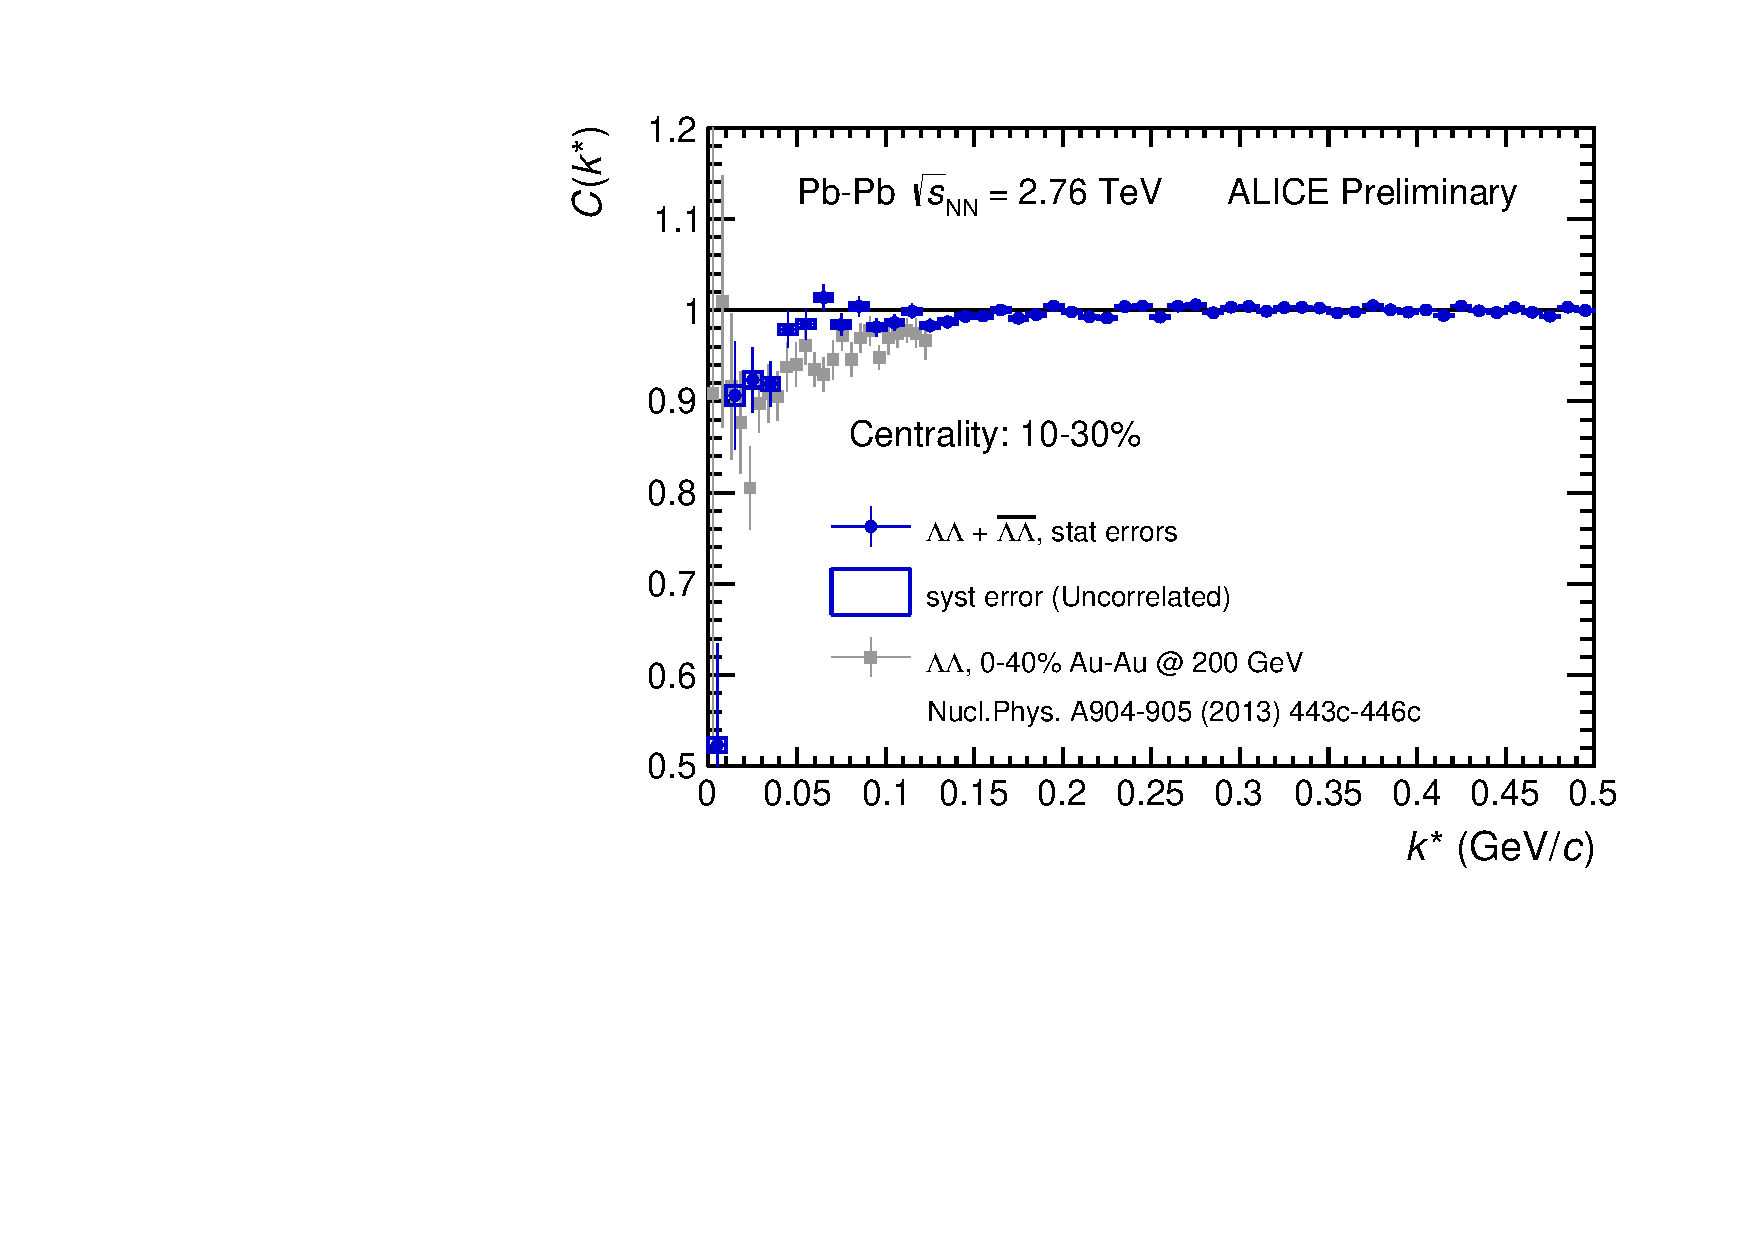
\includegraphics[width=36pc]{Figures/2014-05-11-CfLLAA-1030-CommentCorrections-WithSTAR.pdf}
\caption[$\Lambda\Lambda + \bar{\Lambda}\bar{\Lambda}$ correlation function for the 10-30\% centrality range]{$\Lambda\Lambda + \bar{\Lambda}\bar{\Lambda}$ correlation function for the 10-30\% centrality range with statistical and systematic errors.  A dip at low $k^*$ is seen which is expected from quantum interference.  Preliminary STAR data for $\Lambda\Lambda$ is shown for comparison.  For the same plot without STAR data, see Figure \ref{fig:AppendixCFLamLamALamALam1030}.}
\label{fig:CFLamLamALamALam1030STAR}
\end{figure}
\begin{figure}[hbtp]
\includegraphics[width=36pc]{Figures/2014-05-11-CfLLAA-3050-CommentCorrections.pdf}
\caption[$\Lambda\Lambda + \bar{\Lambda}\bar{\Lambda}$ correlation function for the 30-50\% centrality range]{$\Lambda\Lambda + \bar{\Lambda}\bar{\Lambda}$ correlation function for the 30-50\% centrality range with statistical and systematic errors.  A hint of a dip at low $k^*$ may be seen, which would be expected from quantum interference.}
\label{fig:CFLamLamALamALam3050}
\end{figure}

\begin{figure}[hbtp]
\includegraphics[width=36pc]{Figures/2014-05-11-CfLA-010-CommentCorrections.pdf}
\caption[$\Lambda\bar{\Lambda}$ correlation function for the 0-10\% centrality range]{$\Lambda\bar{\Lambda}$ correlation function for the 0-10\% centrality range with statistical and systematic errors.  A wide suppression is seen which is indicative of annihilative effects.}
\label{fig:CFLamALam010}
\end{figure}
\begin{figure}[hbtp]
\includegraphics[width=36pc]{Figures/2014-05-11-CfLA-1030-CommentCorrections.pdf}
\caption[$\Lambda\bar{\Lambda}$ correlation function for the 10-30\% centrality range]{$\Lambda\bar{\Lambda}$ correlation function for the 10-30\% centrality range with statistical and systematic errors.  A wide suppression is seen which is indicative of annihilative effects.}
\label{fig:CFLamALam1030}
\end{figure}
\begin{figure}[hbtp]
\includegraphics[width=36pc]{Figures/2014-05-11-CfLA-3050-CommentCorrections.pdf}
\caption[$\Lambda\bar{\Lambda}$ correlation function for the 30-50\% centrality range]{$\Lambda\bar{\Lambda}$ correlation function for the 30-50\% centrality range with statistical and systematic errors.  A wide suppression is seen which is indicative of annihilative effects.}
\label{fig:CFLamALam3050}
\end{figure}

\subsection{Interpretation of correlation function results}
\label{sec:CFInterpretation}


Generally speaking, the interesting part of a relative-momentum correlation function is the region below 100 or 200 MeV/c.  Non-unity structures/backgrounds may be visible at large relative momentum - these structures can complicate the fitting procedure, and sometimes even direct attention to flaws in the analysis.  They can also exist in the low-relative momentum region, though there they are generally assumed (or at least hoped) to be small.  However, the information about the source size and two-particle interactions is predominantly encoded within the low-$k^*$ region.  For the time being, this analysis will restrict its attention to behavior in that region.

The $\Lambda\bar{\Lambda}$ correlation functions (Figures\ \ref{fig:CFLamALam010}, \ref{fig:CFLamALam1030}, and \ref{fig:CFLamALam3050}) exhibit a clear, centrality dependent suppression in the low-$k^*$ region, even with the significant statistical error bars for the 10-30\% and 30-50\% systems.  A signal is also visible in the $\Lambda\Lambda + \bar{\Lambda}\bar{\Lambda}$ data, though it is smaller in magnitude and localized to a narrower $k^*$ region. For reference, Preliminary STAR $\Lambda\Lambda$ results from 200 GeV Au--Au, 0-40\% centrality are also plotted \cite{Shah:2012ps}.

Several factors may contribute to the small size of this signal.  First of all, the physics of the identical particle systems (see Sec.\ \ref{sec:AnalyticModel}) is expected to be confined to just the few lowest bins.  There may be competing physics effects -- a suppression from quantum interference and an enhancement from the strong final state interactions -- that wash each other out.  Furthermore, two-track effects like splitting and merging show up in this region, though they are assumed to be well-corrected for by the aforementioned pair-wise cuts.  The presence of residual correlations might muddle or dilute the signal region.  This will be discussed further in Section \ref{sec:Residual}.  Finally, it must be noted that these are the $k^*$ bins with the least statistics.  There are also a couple of fitting tricks that can be employed to mitigate the statistical limitations in these plots.  They will be discussed in Section \ref{sec:MinuitFit}.

%********Outdated****** some of this may be salvageable

%Figure \ref{fig:CFMixCentralities} shows $\Lambda\bar{\Lambda}$ correlation functions versus $q_{\rm inv}$ for three different centralities ranges.  The correlations are normalized to unity in the $ 0.3 < q_{\rm_{inv}} < 0.5$ GeV/c range.  Each correlation shows clear suppression in the low-$q_{\rm_{inv}}$ region, which is considered an effect of the baryon-antibaryon annihilation channel.  The strength of the correlation effect increases with more peripheral events, an indication that the emitting source size is shrinking for those events.

%Figure \ref{fig:CF} shows correlation functions constructed in the 0-10\% centrality range for $\Lambda\Lambda$ and $\bar{\Lambda}\bar{\Lambda}$ pairs.  Both correlation functions exhibit an enhancement in the low-$q_{\rm inv}$ range of 0.04 - 0.2 GeV/c.  This may be due to attractive final state interactions.  The effects of FSI and quantum statistics are expected to be seen in roughly the same $q_{\rm inv}$ range, and it is unclear at this time to what extent their effects should be competing. The enhancement of the $\bar{\Lambda}\bar{\Lambda}$ correlation function does fall off in the lowest bins, though the statistical uncertainties are such that no significant statement about the effects of quantum statistics can be made at this time.



\section{1D analytic model}
\label{sec:AnalyticModel}
%\subsection{Analytical model}
With the assumption of a spherically gaussian source of width $R$, the 1D femtoscopic correlation functions can be calculated analytically \cite{lednicky82} using 

\begin{equation}
C(k^*)= 1 + C_1(k^*)+C_2(k^*).
\end{equation}
$C_1$ describes plane-wave quantum interference:
\begin{equation}
C_1(k^*) = \alpha e^{-4k^{*2}R^2}
\end{equation}
where $\alpha = (-1)^{2j}/(2j+1)$ for identical particles with spins $j$, and $\alpha = 0$ for non-identical particles.  $C_2$ describes the s-wave strong final state interaction of the particles:
\begin{equation}
\label{eq:Lednicky}
C_2(k^*)= (1+\alpha)\left[\frac{1}{2}\abs{\frac{f(k^*)}{R}}^2(1-\frac{d_0}{2\sqrt{\pi}R})+\frac{2\Re f(k^*)}{\sqrt{\pi}R}F_1(2k^*R)-\frac{\Im f(k^*)}{R}F_2(2k^*R)\right]
%C_2(k^*)= 1+ \displaystyle\sum\limits_{S}\rho_S\left[\frac{1}{2}\abs{\frac{f^S(k^*)}{R}}^2(1-\frac{d_0^S}{2\sqrt{\pi}R})+\frac{2\Re f^S(k^*)}{\sqrt{\pi}R}F_1(2k^*R)-\frac{\Im f^S(k^*)}{R}F_2(2k^*R)\right]
\end{equation}
where $F_1(z) = \int_0^z \! \mathrm{d}x \, e^{x^2-z^2}/z$,  $F_2(z) = (1-e^{-z^2})/z$, and $R$ is the source size. The $(1+\alpha)$ pre-factor accounts for the relevant (non/anti-)symmetrizaton effects.  $f(k^*)=(1/f_0+\frac{1}{2}d_0k^*-ik^*)^{-1}$ is the s-wave scattering amplitude, written using the effective range approximation.  The scattering amplitude is dependent upon the effective range of interaction $d_0$, as well as the complex scattering length $f_0$.  The real part of the scattering amplitude can contribute either a positive or a negative correlation, but either way the effect is relatively narrow in $k^*$ (on the order of about one hundred MeV/$c$).  The imaginary part of the scattering amplitude accounts for inelastic processes of baryon-antibaryon annihilation.  Introducing a non-zero imaginary part to the scattering length produces a wide (hundreds of MeV/$c$) negative correlation.  For charged particles, an additional factor \cite{Aamodt:2011kd} is necessary to account for the Coulomb interaction.

Technically, the scattering length and effective range are spin dependent.  It should be noted that in the case of identical fermions, "the contributions of s-wave interaction of identical nucleons to the correlation function goes to zero [for summary spin state S = 1] (identical nucleons with parallel spins cannot be in the s-wave state)" \cite{lednicky82}.  As a result, only the spin singlet (i.e. antisymmetric spinor, symmetric spatial wave function) scattering parameters are measured for identical fermions.  Such is the case for the $\Lambda\Lambda$ and $\bar{\Lambda}\bar{\Lambda}$ correlation measurements.  However, for non-identical particles such as $\Lambda\bar{\Lambda}$, the factor $(1+\alpha)$ could be replaced with a weighted sum of $C_2$ calculated using separate spin-dependent scattering parameters.  That calculation would use $\rho_S$, the fraction of pairs in each total spin state S, as the weight.  For statistical reasons, this analysis will eschew spin-dependent measurements of the $\Lambda\bar{\Lambda}$ scattering parameters, and instead attempt to fit for a spin-averaged value.


\subsection{Observables}
\label{sec:Observables}
For pion, kaon, and proton femtoscopic analyses, the scattering lengths and effective radius of interaction are well specified by years of scattering data, and they can be fixed to the known values.  In the case of lambda-(anti-)lambda femtoscopy, the interaction is heretofore largely unstudied.  For this analysis, the scattering lengths and effective radius are left as free parameters.  Another free parameter is the $\lambda$ parameter, which is roughly a measure of the pair purity.  For example, $\lambda_{\Lambda\Lambda}$ would correspond to the ratio of number of true primary $\Lambda\Lambda$ pairs to the total number of pairs in the correlation function. The remaining fraction is comprised of all the other combinations of pair types, such as pairs where one $\Lambda$ is real and primary and the other is fake, or pairs between primary and secondary lambdas.  The latter case will be described further in Section \ref{sec:Residual}.  The last fit parameter is $R_{\rm inv}$, which characterizes the one dimensional size of the emitting source.  


\section{Residual correlations}
\label{sec:Residual}

Attempts at fitting correlation functions should try to account for residual correlations between the particle being studied and other particles that might decay into the studied particle.  Various particles can decay into $\Lambda$ baryons, such as $\Sigma^{\rm 0}$, $\Xi^{\rm 0}$, and $\Omega^{\rm -}$.  The decay momentum difference between these particles and their daughter $\Lambda$ is small, such that daughter and parent carry very similar momenta.  As a result, relative-momentum correlation functions between primary particles and secondary particles can be sensitive to the interactions between the primary particles and the parent particles.  For example, the correlation between primary $\Lambda$ and primary $\Sigma^{\rm 0}$ should be visible, though somewhat smeared out, in the correlation between primary $\Lambda$ and secondary $\Lambda$.  Furthermore, these secondary $\Lambda$ are often difficult to distinguish from primary $\Lambda$.  Therefore, measurements of two-$\Lambda$ correlation functions will contain a mixture of primary correlations and feeddown correlations, and an attempt to parametrize the correlation functions should take this into account.  

In this analysis note, we will discuss two different methods of accounting for these residual correlations.  In the "Transformed residuals method", the Lednicky equation is used to estimate the shape of the residual correlations \emph{before} they decay (e.g. to estimate the shape of the $\Lambda\Sigma$ correlation function in the $\Lambda\Sigma$ relative momentum space).  This pre-feeddown correlation is then smeared into a residual correlation function (in the $\Lambda\Lambda$ momentum space) using a transform matrix that accounts for the kinematic effects of the decay of one or both of the particles.  Different sources of residual correlations are determined separately and then summed together with the primary-primary correlation in the fit procedure.

In contrast, the "Gaussian residuals method" attempts to describe the full residual correlation effect phenomenologically.  Rather than precisely describe each component of residual correlation, the total residual correlation is described with a Gaussian parametrization.  %In essence, the residual correlations described by the transform method are roughly Gaussian, so the Gaussian parametrization 


\subsection{Transformed residuals method}
\label{sec:TransformedResiduals}


One example of transformed residuals parametrization can be seen in the recent analysis \cite{Kisiel:2014mma} of STAR p$\bar{\Lambda}$ correlation functions measured in 200 GeV Au--Au collisions.  In this study, p$\bar{\Lambda}$ and $\bar{\mathrm{p}}\Lambda$ correlations were fit with and without residual correlations.  The fits with residual correlations included feeddown and feedup contributions from numerous sources.  The study found that the fit with residual correlations measured a source size comparable to the previously measured sizes of p$\Lambda$ and $\bar{\mathrm{p}}\bar{\Lambda}$.  In contrast, the fits that did not include residual correlations measured source radii that deviated significantly from the old p$\Lambda$ and $\bar{\mathrm{p}}\bar{\Lambda}$ results.  One conclusion from that study was that it is important to make a precise characterization of the $\lambda$ parameters associated with each type of pair contribution.  As mentioned above in Section \ref{sec:Observables}, the $\lambda$ parameter can be interpreted as the fraction of total pairs associated with that pair type.  Quantitatively, it is included in the fit as shown in Equation \ref{eq:Residual} below.

We attempt to quantify the residual contamination in this analysis by simultaneously fitting the data for both the primary correlation function and the residual correlations.  For example, $\Lambda\Lambda$ correlations with $\mathrm{\Lambda\Sigma^0}$ feeddown would be fit using 

\begin{equation}
\label{eq:Residual}
C_{\mathrm{meas}}(k^*_{\Lambda\Lambda})= 1 + \lambda_{\Lambda\Lambda}[C_{\Lambda\Lambda}(k^*_{\Lambda\Lambda})-1]+\lambda_{\Lambda\Sigma}[C_{\Lambda\Sigma}(k^*_{\Lambda\Lambda})-1],
\end{equation}
where $$C_{\Lambda\Sigma}(k^*_{\Lambda\Lambda}) \equiv \displaystyle\sum\limits_{k^*_{\Lambda\Sigma}}C_{\Lambda\Sigma}(k^*_{\Lambda\Sigma})T(k^*_{\Lambda\Sigma},k^*_{\Lambda\Lambda}),$$ $C_{\Lambda\Sigma}(k^*_{\Lambda\Sigma})$ is the $\Lambda\Sigma$ correlation function calculated from Eq.~(\ref{eq:Lednicky}), and $T$ is a THERMINATOR \cite{Chojnacki:2011hb} transform matrix, which shows how the $k^*$ of pairs of particles kinematically transforms when one of the particles decays.  Figure \ref{fig:TherminatorLS} shows the transform matrix for $\Lambda\Sigma \rightarrow \Lambda\Lambda$.  In this simple case with only two pair types ($\Lambda\Lambda$ and $\Lambda\Sigma$), the $\lambda$ parameters could either be fixed to some estimated experimental value, or they could be left as free fit parameters.

\begin{figure}[hbtp]
\includegraphics[width=36pc]{Figures/2014-04-01-TransformMatrix-LS-LL-100bins.pdf}
\caption[Transform matrix for $k^*_{\Lambda\Sigma} \rightarrow k^*_{\Lambda\Lambda}$]{THERMINATOR \cite{Chojnacki:2011hb} transform matrix showing how the relative momentum of $\Lambda\Sigma$ pairs transforms into relative momentum of $\Lambda\Lambda$ pairs after the $\Sigma$ decays.  The elements significantly off-diagonal may be due to a lingering bug in the construction of the transform matrix.}
\label{fig:TherminatorLS}
\end{figure}

Further residual correlations (e.g. from $\Sigma\Sigma \rightarrow \Lambda\Lambda$) can be included via additional terms in Equation \ref{eq:Residual}.  Efforts are under way to understand which residual correlations must be included and which can be safely neglected.  Section \ref{sec:LambdaParams} will discuss the current status of this analysis. 

\subsection{Gaussian residuals method}
\label{sec:GaussianResiduals}

The Gaussian residuals method has also been used \cite{Shapoval:2014yha} to fit the STAR p$\bar{\Lambda}$ data.

In the Gaussian residual method, the measured correlation function is fit with 

\begin{equation}
\label{eq:GaussianResiduals}
C_{\mathrm{meas}}(k^*) = \lambda_{\mathrm{prim}}*C_{\mathrm{prim}}(k^*)+(1-\lambda_{\mathrm{prim}})(1-\beta  e^{-4k^{*2}\omega^2})
\end{equation}

%advantages: Don't need to know/make big assumptions about residual interaction parameters.

%disadvantages:  Hard to interpret fit parameters.  Might conflict 

\section{Fitting results and systematics}
\label{sec:FittingSystematics}



\subsection{Fitting via Gaussian residual method}



\subsection{Fitting via the transform method}

Proper fitting techniques for this analysis are still a work in progress.  In particular, efforts are being made to evaluate the extent to which residual correlations permeate the measured correlation functions.  In this analysis, the importance of residual correlations can be characterized by two sets of parameters.  The scattering lengths $f_0$ of the residual pair describe the strength of the residual pair interaction, such that a larger $\abs{f_0}$ will generally lead to a more pronounced residual correlation function.  Meanwhile, the pair purity $\lambda$ of each pair type describes the relative contribution of each individual correlation function (i.e. primary or residual) to the total correlation function, as described in Section \ref{sec:Residual}. The following sections will discuss how these two parameters are evaluated in this analysis.


%Discussion of current status of fit results and systematic uncertainties.  Report measured systematics as well as possible sources of systematics yet to be explored.

\subsection{Estimates of $\lambda$ parameters}
\label{sec:LambdaParams}

In this section, we attempt to make a very rough, preliminary estimate of the relevant $\lambda$ parameters involved in this calculation.  A more refined estimate could be made by convoluting ALICE particle spectra with analysis-specific reconstruction efficiencies to determine analysis-specific yields of the various particle types.  That avenue will be discussed more in Section \ref{sec:ReconstructionEff}. 

To understand the mathematical motivation behind the $\lambda$ parameters, let us consider the simple case where the signal pairs of the correlation function come from a single event.  Within this event, all combinations of reconstructed V0s are paired together and binned according to their $k^*$ values.  For this analysis, the reconstructed V0s consist of primary $\Lambda$, secondary $\Lambda$, and false $\Lambda$.  Let us assume that origin of the different $\Lambda$ cannot be determined - the analysis only knows that a given V0 appears to be a $\Lambda$.  As mentioned above, the total correlation function will be a linear combination of the component correlation functions (primary-primary, primary-secondary, primary-fake, fake-fake, etc.).  The $\lambda$ parameters for each component correlation are given by the fraction of total pairs of that type.  For example, if there are ten distinct $\Lambda\Sigma$ pairs and one hundred total pairs, then $\lambda_{\Lambda\Sigma} = 1/10$.  Ideally, the sum of all $\lambda$ should be unity.  That said, in practice one reason the sum of $\lambda$ parameters can deviate from unity is if the source is not truly a gaussian.

The following equations describe a combinatoric approach for estimating the $\lambda$ parameters for different types of pairs.  For two identical particles (e.g. primary $\Lambda$) \begin{equation}
\label{eq:LambdaIdentical}
\lambda_{\Lambda\Lambda} = \frac{N_\Lambda}{T}\frac{(N_\Lambda -1)/2}{(T-1)/2} = \frac{N_\Lambda}{T}\frac{(N_\Lambda -1)}{(T-1)}
\end{equation}
where the $\Lambda$ subscript means primary $\Lambda$, $N$ is the number of particles of that type, $T$ is the total number of all indistinguishable particles, and the factors of $1/2$ remove double counting.  For two different, indistinguishable particles (e.g. a primary $\Lambda$ and a $\Lambda$ from a $\Sigma^0$ decay)
\begin{equation}
\lambda_{\Lambda\Sigma} = \frac{N_\Lambda}{T} \frac{N_\Sigma}{(T-1)/2}
\end{equation}
where the $\Sigma$ subscript indicates $\Lambda$ from $\Sigma$ decays.  $\lambda$ can also be calculated for pairs that are distinguishable, such as primary $\Lambda$ and primary $\bar{\Lambda}$:
\begin{equation}
\lambda_{\Lambda\bar{\Lambda}} = \frac{N_\Lambda}{T_{\Lambda-\mathrm{type}}} \frac{N_{\bar{\Lambda}}}{T_{\bar{\Lambda}-\mathrm{type}}}
\end{equation}
where $T_{\Lambda-\mathrm{type}}$ is the sum of all indistinguishable particles that look like $\Lambda$, etc.  These equations are all easily generalized to other particle pairs.

One should note here that the above $\lambda$ equations technically apply to some sort of single-event correlation function.  The $\lambda$ parameters measured or estimated for a million-event correlation function would roughly correspond to an event-averaged value.  Nonetheless, we can attempt to employ these formulae to obtain ballpark estimates of the $\lambda$ parameters, given estimates of the yields of each type of particle.

As the goal of this analysis is to measure the correlations of primary $\Lambda$, it is important to know the relative yields of secondary $\Lambda$.  We can obtain an estimate \cite{Florkowski:2010zz} of the yields of different types of particles at mid-rapidity from a thermal model using
\begin{equation}
\frac{1}{m_{\mathrm{T}}}\frac{dN}{dm_{\mathrm{T}}} \propto \exp{(-m_\mathrm{T}/T)}
\end{equation}
where the transverse mass $m_\mathrm{T} = \sqrt{m^2_{\mathrm{inv}} + p^2_{\mathrm{T}}}$ and $T$ is the chemical-feezeout temperature.  Integrating over $m_\mathrm{T}$ gives $N \propto (m_\mathrm{inv} + T) \exp{(-m_\mathrm{inv}/T)}$.  Therefore, the yield of any particle species $i$ relative to the $\Lambda$ yield is
\begin{equation}
\frac{N_i}{N_\Lambda} \approx \frac{m_i + T}{m_\Lambda + T} \exp{((m_\Lambda - m_i)/T)}.
\end{equation}

Particles that decay into $\Lambda$ include $\Sigma^0$, $\Xi^0$, $\Xi^-$, and $\Omega^-$.  Assuming a freezeout temperature of 165 MeV, and taking into account that the $\Omega$ has a branching ratio of ~68\% and the others ~100\%, we can then estimate that for every 100 $\Lambda$, there will be approximately 67 $\Sigma$, 34 of each type of $\Xi$, and 3 $\Omega$.

Before calculating the $\lambda$ parameters, it is also necessary to know approximately how many fake $\Lambda$ there are.  In Section \ref{sec:Recon}, we estimated that our signal quality $P$ was $P = real/(real + background) \approx 0.82$ (Note: calculations were performed using a now outdated purity estimate).  Taking $real$ to be the sum of all the primary and secondary $\Lambda$, we calculate that $\frac{background}{real} = P^{-1}-1 \approx 0.22$.  With the above yields totalling 238 $\Lambda$, we would expect to see an additional 52 fake $\Lambda$.  Based on these values, we can now estimate the $\lambda$ parameters for all pair types.

\begin{center}
\begin{tabular}{|l|l|c|}
\hline
					& 	$\lambda$	&	Cumulative total \\ \hline
$\Lambda\Lambda$   	&	0.12			&	0.12 \\ \hline
$\Lambda\Sigma^0$  	&	0.16			&	0.28 \\ \hline
$\Lambda\Xi^0$     	&	0.08			&	0.36 \\ \hline
$\Lambda\Xi^-$     	&	0.08			&	0.44 \\ \hline
$\Lambda\Omega$    	&	0.007		&	0.45 \\ \hline
$\Sigma^0\Sigma^0$ 	&	0.05			&	0.50 \\ \hline
$\Sigma^0\Xi^0$    	&	0.05			&	0.55 \\ \hline
$\Sigma^0\Xi^-$    	&	0.05			&	0.61 \\ \hline
$\Sigma^0\Omega$   	&	0.004		&	0.61 \\ \hline
$\Xi^0\Xi^0$       	&	0.01			&	0.63 \\ \hline
$\Xi^0\Xi^-$ 		&	0.03			&	0.65 \\ \hline
$\Xi^0\Omega$ 		&	0.002		&	0.66 \\ \hline
$\Xi^-\Xi^-$ 		&	0.01			&	0.67 \\ \hline
$\Xi^-\Omega$ 		&	0.002		&	0.67 \\ \hline
$\Omega\Omega$ 		&	0.00			&	0.67 \\ \hline
\end{tabular}
\end{center}

These estimates have several interesting characteristics.  First, the sum of the primary correlation all the residual correlations totals to 0.67.  The other 33\% is lost to the background.  Note that feedup from residual p$\Lambda$ correlations would be included in this 33\%, though feedup has otherwise not yet been explored in this analysis. Another striking feature of these data is that the contribution from $\Lambda\Sigma$ is actually larger than the contribution from $\Lambda\Lambda$.  In other words, if the hyperon yields and reconstruction efficiencies of the true PbPb data are reminiscent of the yields above, then this analysis is measuring the $\Lambda\Sigma$ correlation more than the $\Lambda\Lambda$ correlation.  It should also be noted that contributions from $\Lambda\Xi$, $\Sigma\Sigma$, and $\Sigma\Xi$ are appreciable.

For the the $\Lambda\bar{\Lambda}$ analysis, estimates of the $\lambda$ parameters work out to be approximately the same as in the table above.

\subsection{Reconstruction efficiency effects on relative particle yields}
\label{sec:ReconstructionEff}

Note: This section is still under construction.  While the details eventually contained here will be important for fitting correlation functions, these details not particularly relevant for the construction of the correlation functions (i.e. the results under approval for Quark Matter 2014).  The plots have yet to be finalized - they will be added later.

The above $\lambda$ estimates have been made under the assumption that primary and secondary $\Lambda$ have the same chance to be reconstructed.  However, detector efficiencies and topological reconstruction cuts can change the relative yields of each of these $\Lambda$ types.  To investigate the influence of reconstruction efficiencies on particle yields, we looked at the reconstruction rates of the different particle types using the HIJING run specified in Section \ref{sec:DataSelection}.  The MC truth yields of the V0s were examined at three stages of reconstruction:
\begin{itemize}
\item In the raw MC event before any detector simulation was added to the MC particles.  Here the daughters of the V0s are required to be in mid-rapidity and surpass a minimum $p_\mathrm{T}$ value.
\item In the V0 finder before any analysis-side reconstruction cuts were employed.
\item After topological reconstruction cuts were made.
\end{itemize}
At each stage, the MC truths of all remaining particles of the following types were counted: primary $\Lambda$; secondary $\Lambda$ from $\Sigma^0$, $\Sigma^*$, $\Xi^0$, $\Xi^-$, $\Omega$, and other sources; the respective anti-particles; $\mathrm{K}^0_{\mathrm{S}}$ misidentified as $\Lambda$ or $\bar{\Lambda}$; other misidentified V0s; and fake V0s reconstructed in the V0 finder.  The resulting yields are visible in Figure \ref{fig:MCYields}.

The results of Figure \ref{fig:MCYields} can be better interpreted by taking the ratios of the yields at different stages.  Figure \ref{fig:V0ToMassCut} shows one such ratio.  Here, one can see the fraction of V0s in the V0 finder that survived all the reconstruction cuts.  From this, one can see how successful the current topological cuts are at selecting (anti)$\Lambda$ of various origins.  With different topological cuts made, a before-and-after comparison of this plot shows the efficacy of the new cuts at removing secondary V0s vs primary V0s, as in Figure \ref{V0ToMassCutWithDifferentVarBin}.

Figure \ref{fig:OriginToMassCut} shows another ratio.  In this plot, one sees the event-averaged reconstruction efficiency from the beginning (particles in the underlying event) to the end (all particles passing all cuts).  This efficiency encompasses not only the results of the analysis-side cuts, but also the natural tracking efficiencies of ALICE detector.  One can see that the various $\Lambda$ and $\bar{\Lambda}$ types for the most part have a reconstruction rate between 15-25\%.  These reconstruction efficiencies could be convoluted with the thermal yield calculations of Section \ref{sec:LambdaParams} to obtain corrected estimates of the yields and $\lambda$ parameters.  Further analyses of these results are in progress.

\subsection{A note on injected Monte Carlo signals}
\label{sec:InjectedMCSignals}

It should be noted that this MC run, LHC12a17a\_fix, has injected $\Xi^0$, $\Xi^-$, and $\Omega$ signals, but not their respective antiparticles.  The disparity can be seen in Figure \ref{fig:MCEfficiencyWithInjected}, which shows the average reconstruction efficiencies of $\Lambda$ ($\bar{\Lambda}$) broken down in terms of the Monte Carlo truth of each V0's parent species. The reconstruction efficiency is defined as the ratio of the number of reconstructed $\Lambda$ ($\bar{\Lambda}$) of each origin type versus the number of V0 candidates of each origin in the V0 finder.  A clear disparity can be seen between the reconstruction efficiencies of $\Lambda_{\Xi}$ and $\Lambda_{\Omega}$ and their respective antiparticles.  (This plot is a few months out of date - the reconstruction cuts employed in this figure are somewhat looser than those employed in the current analysis.)

The origin of this disparity has not been investigated in great detail, though it is suspected that the disparity arises from differences between the $p_\mathrm{T}$ spectra of the injected V0s and the 
underlying HIJING particles.  Because the efficacy of the various reconstruction cuts and the detector efficiency is $p_\mathrm{T}$ dependant, the average reconstruction efficiency of injected particles may differ from the base HIJING particles.  Figure \ref{fig:MCEfficiencyWithInjected} therefore shows a disparity between multistrange hyperon and antihyperon efficiency because the hyperons include a mix of injected and underlying particles, while the antihyperons come only from the underlying event. The analysis was performed again with injected signals removed (see Figure \ref{fig:MCEfficiencyNoInjected}).  Without the injected signals, reconstruction efficiencies for the multi-strange particles and anti-particles are seen to be in line.  Subsequent studies of reconstruction cuts and efficiency were performed without injected signals such that secondary $\Lambda$ and $\bar{\Lambda}$ efficiencies would be consistent.

\begin{figure}[hbtp]
\includegraphics[width=36pc]{Figures/2014-04-20-Efficiency-WithInjectedSignals-OldCuts_2013-09-04Run.pdf}
\caption[$Lambda$ reconstruction efficiencies with injected signals]{Average reconstruction efficiencies of $\Lambda$ ($\bar{\Lambda}$) broken down in terms of the Monte Carlo truth of each V0's parent species.  Reconstruction efficiency is defined as the ratio of the number of reconstructed $\Lambda$ ($\bar{\Lambda}$) of each origin type versus the number of V0 candidates of each origin in the V0 finder.  The analysis was performed for HIJING events with injected hyperon signals.  The events included injected $\Lambda$, $\bar{\Lambda}$, $\Xi$, and $\Omega$, but no $\bar{\Xi}$ or $\bar{\Omega}$.  A clear disparity can be seen between the reconstruction efficiencies of $\Lambda_{\Xi}$ and $\Lambda_{\Omega}$ and their respective antiparticles.  This plot is a few months out of date - the reconstruction cuts employed in this figure are somewhat looser than those employed in the current analysis.}
\label{fig:MCEfficiencyWithInjected}
\end{figure}

\begin{figure}[hbtp]
\includegraphics[width=36pc]{Figures/2014-04-20-Efficiency-NoInjectedSignals-OldCuts_2013-11-19Run.pdf}
\caption[$Lambda$ reconstruction efficiencies without injected signals]{Average reconstruction efficiencies of $\Lambda$ ($\bar{\Lambda}$) broken down in terms of the Monte Carlo truth of each V0's parent species.  Reconstruction efficiency is defined as the ratio of the number of reconstructed $\Lambda$ ($\bar{\Lambda}$) of each origin type versus the number of V0 candidates of each origin in the V0 finder.  The analysis was performed for HIJING events with injected hyperon signals.  However, injected hyperon signals have been excluded from this plot.  The various secondary $\Lambda$ are seen to have approximately the same reconstruction efficiency as respective antiparticles.  This plot is a few months out of date - the reconstruction cuts employed in this figure are somewhat looser than those employed in the current analysis.}
\label{fig:MCEfficiencyNoInjected}
\end{figure}

\subsection{Scattering parameters of residual pairs}
\label{sec:ScatteringParams}

As previously mentioned, little information exists about the hyperon-hyperon scattering parameters.  One goal of this analysis is to make a measurement of the $\Lambda\Lambda$ scattering lengths and effective radius.  However, the task remains to decide how to deal with the scattering parameters of all the various residual correlations, which are equally unknown.  One option would be to include separate parameters for each pair interaction.  However, this would introduce two or three new parameters (for particle-particle or particle-antiparticle, respectively) per pair type and yield a very unconstrained fit.  Another option would be to tighten cuts to remove as many of the secondary $\Lambda$ as possible.  However this route stands to significantly reduce the statistics of the fit, as primary $\Lambda$ will be lost alongside the secondary.  On top of that, reconstruction cuts are unlikely to appreciably cut out $\Sigma$ daughters, as the electromagnetic decay of the $\Sigma$ comes with a very short decay length.

Yet another option would be to ansatz that all the pairs interact with approximately the same strength as the $\Lambda\Lambda$ interaction.  The disadvantage of this method is that the final measurement will essentially yield a weighted average of the various pair scattering parameters.  However, the advantage is that it allows all pairs (primary-primary, primary-secondary, secondary-secondary) to provide relevant contributions to the correlation function.  One potential way to estimate the systematic uncertainties in this method would be to do several additional fits, wherein the scattering parameters of the other pairs are treated as being 50\%, 25\%, and 0\% (no interaction) the strength of the $\Lambda\Lambda$ parameters.

\subsection{Minuit fitting}
\label{sec:MinuitFit}

%Include practical treatment of fit parameters here. Residual correlation scattering lengths, simultaneous fitting.  Normalization factor vs polynomial background.
Discussion of Minuit fitting procedure will go here.

\subsection{Fit systematics}
\label{sec:FitSystematics}

Discussion of fit systematics will go here.

\subsection{Fit results and interpretation}
\label{sec:FitResults}

Interpretation of final fit results will go here.

\section{Summary}
Results have been shown for correlation functions $\Lambda\Lambda$, $\bar{\Lambda}\bar{\Lambda}$ and $\Lambda\bar{\Lambda}$ pairs.  The low- to mid-$k^*$ suppression of the $\Lambda\bar{\Lambda}$ correlations in each of the three centrality bins may indicate pair annihilation processes reminiscent of those reported in other studies.

\section{Appendix}
\subsection{Plots for Quark Matter 2014 approval}
\begin{figure}[hbtp]
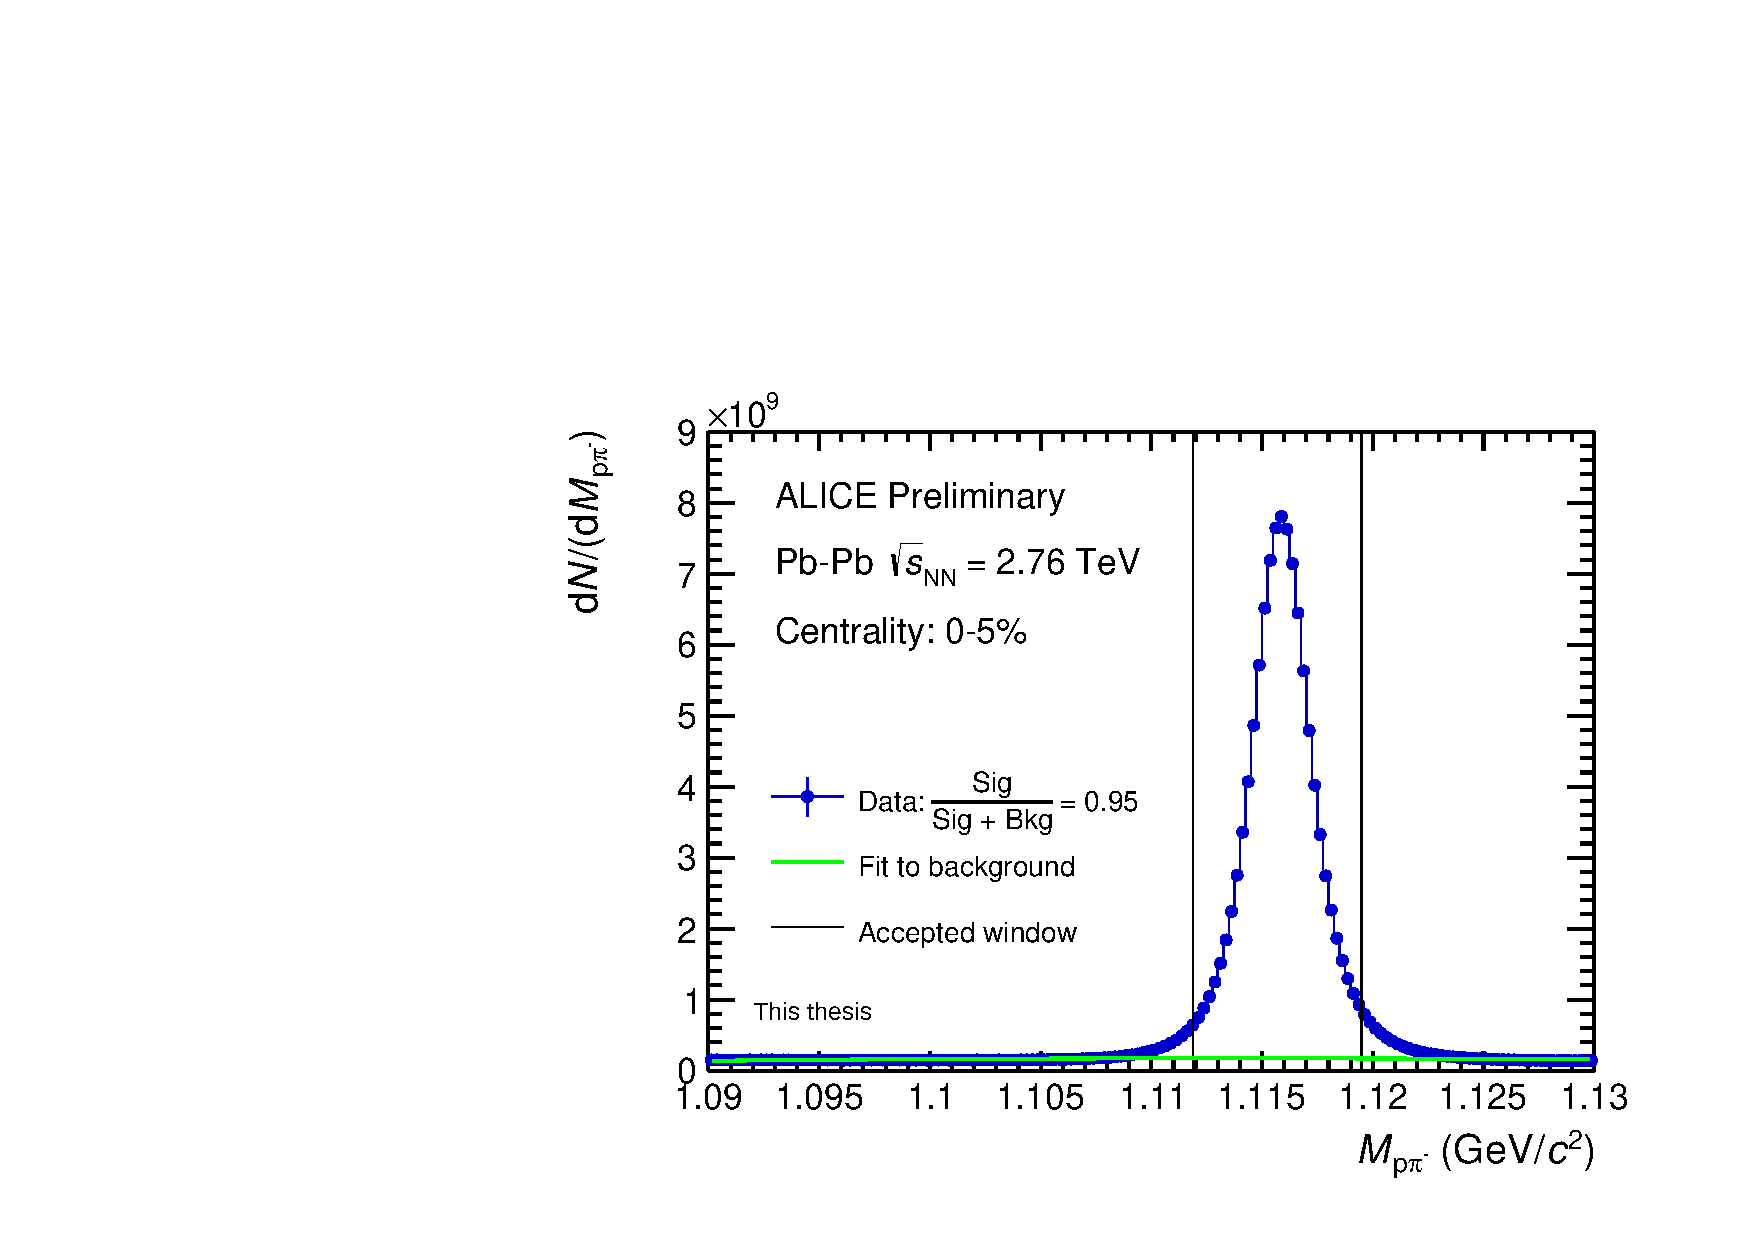
\includegraphics[width=36pc]{Figures/2014-05-11-LamMinv-CommentCorrections.pdf}
\caption[$\Lambda$ invariant mass distribution]{Invariant mass distribution for reconstructed $\Lambda$ using the optimal analysis cuts.  The plots show V0s reconstructed from centrality integrated LHC11h data.  The green line shows a fourth order polynomial fit to the background, which is used to estimate the number of real and fake $\Lambda$.  The estimated ratio of real $\Lambda$ to all reconstructed $\Lambda$ in the signal region ($ \lvert m_{\mathrm{inv}} - m_{\mathrm{PDG}}\rvert < 3.8$ MeV/$\rm c^2$) is approximately 0.95.}
\label{fig:AppendixLamInvMass}
\end{figure}

\begin{figure}[hbtp]
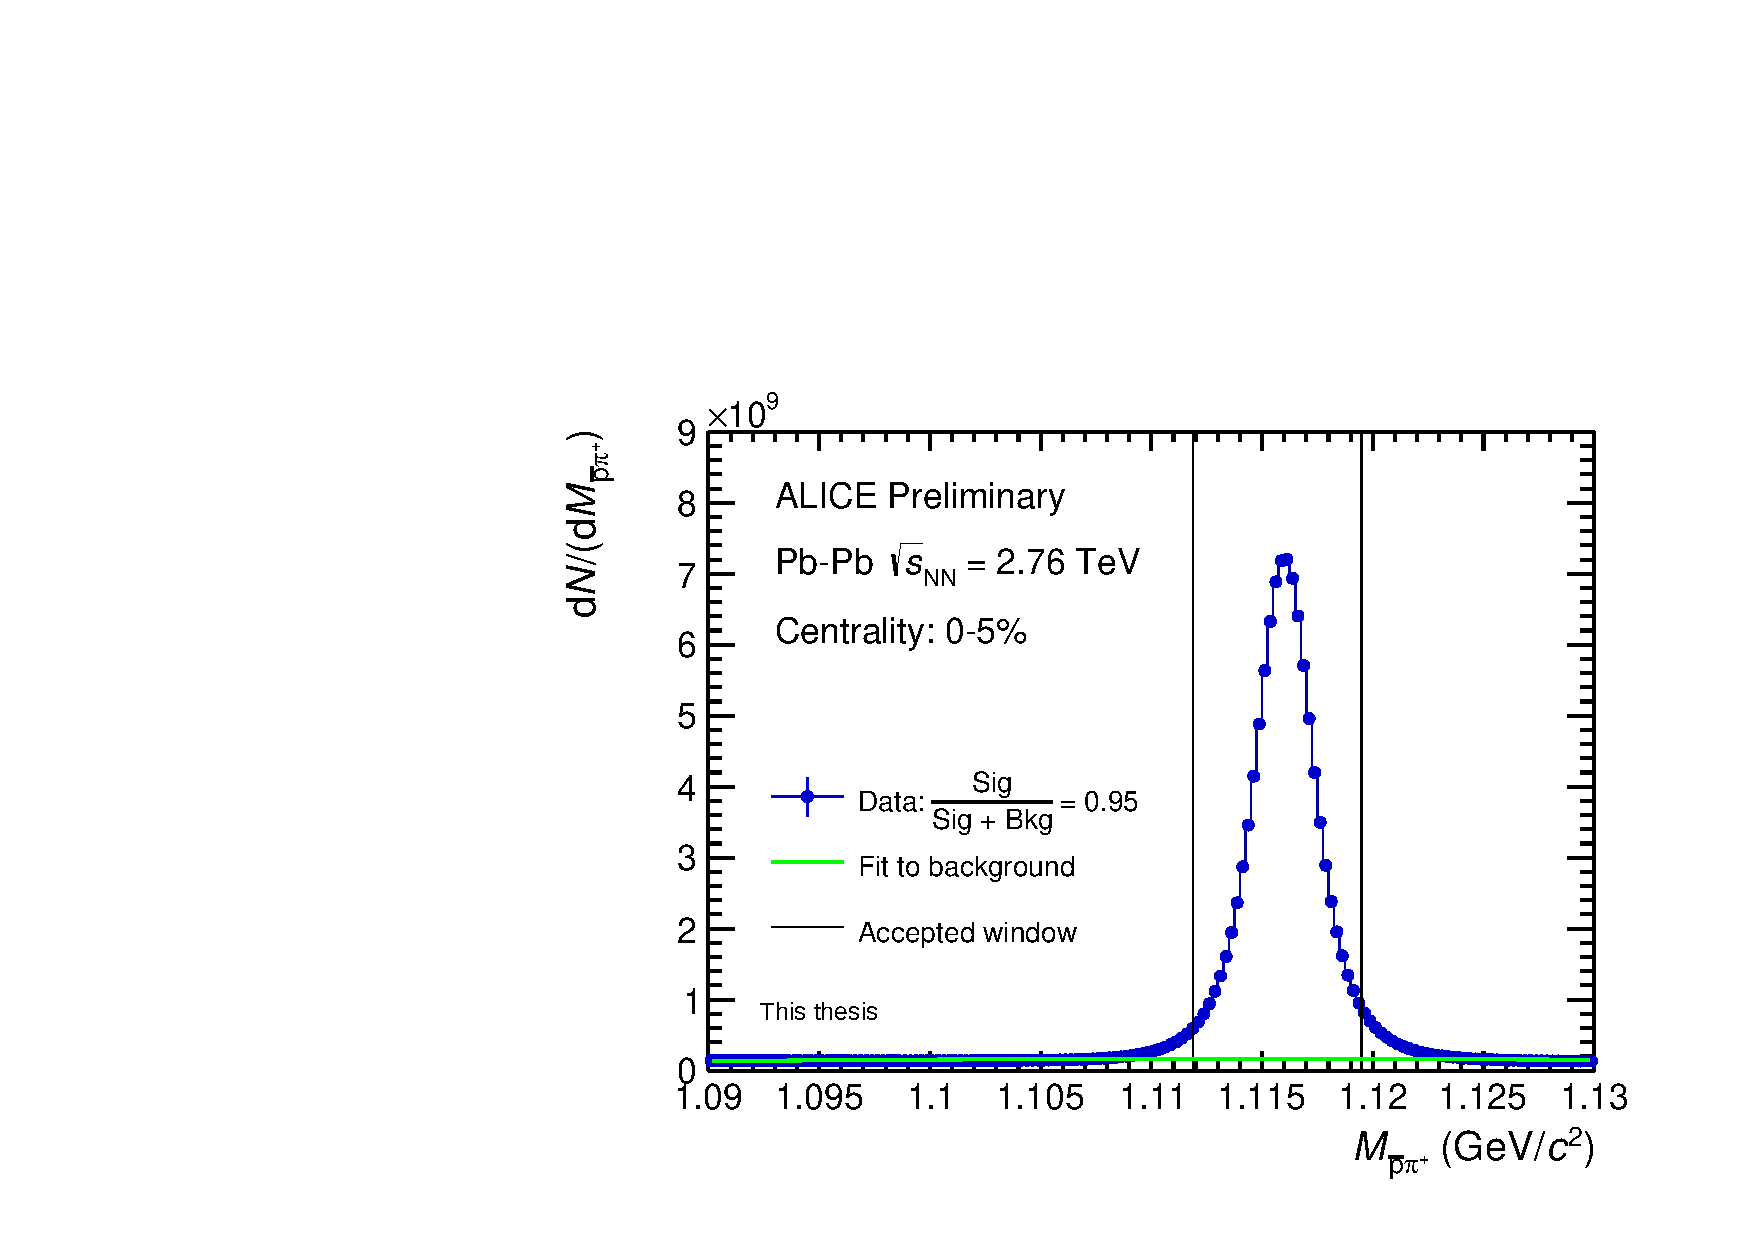
\includegraphics[width=36pc]{Figures/2014-05-11-ALamMinv-CommentCorrections.pdf}
\caption[$\bar{\Lambda}$ invariant mass distributions]{Invariant mass distribution for reconstructed $\bar{\Lambda}$ using the optimal analysis cuts.  The plots show V0s reconstructed from centrality integrated LHC11h data.  The green line shows a fourth order polynomial fit to the background, which is used to estimate the number of real and fake $\bar{\Lambda}$.  The estimated ratio of real $\bar{\Lambda}$ to all reconstructed $\bar{\Lambda}$ in the signal region ($ \lvert m_{\mathrm{inv}} - m_{\mathrm{PDG}}\rvert < 3.8$ MeV/$\rm c^2$) is approximately 0.95.}
\label{fig:AppendixALamInvMass}
\end{figure}

\begin{figure}[hbtp]
\includegraphics[width=36pc]{Figures/2014-05-11-CfLLAA-010-CommentCorrections.pdf}
\caption[$\Lambda\Lambda + \bar{\Lambda}\bar{\Lambda}$ correlation function for the 0-10\% centrality range]{$\Lambda\Lambda + \bar{\Lambda}\bar{\Lambda}$ correlation function for the 0-10\% centrality range with statistical and systematic errors.  A dip at low $k^*$ is seen which is expected from quantum interference.}
\label{fig:AppendixCFLamLamALamALam010}
\end{figure}
\begin{figure}[hbtp]
\includegraphics[width=36pc]{Figures/2014-05-11-CfLLAA-1030-CommentCorrections.pdf}
\caption[$\Lambda\Lambda + \bar{\Lambda}\bar{\Lambda}$ correlation function for the 10-30\% centrality range]{$\Lambda\Lambda + \bar{\Lambda}\bar{\Lambda}$ correlation function for the 10-30\% centrality range with statistical and systematic errors.  A dip at low $k^*$ is seen which is expected from quantum interference.}
\label{fig:AppendixCFLamLamALamALam1030}
\end{figure}
\begin{figure}[hbtp]
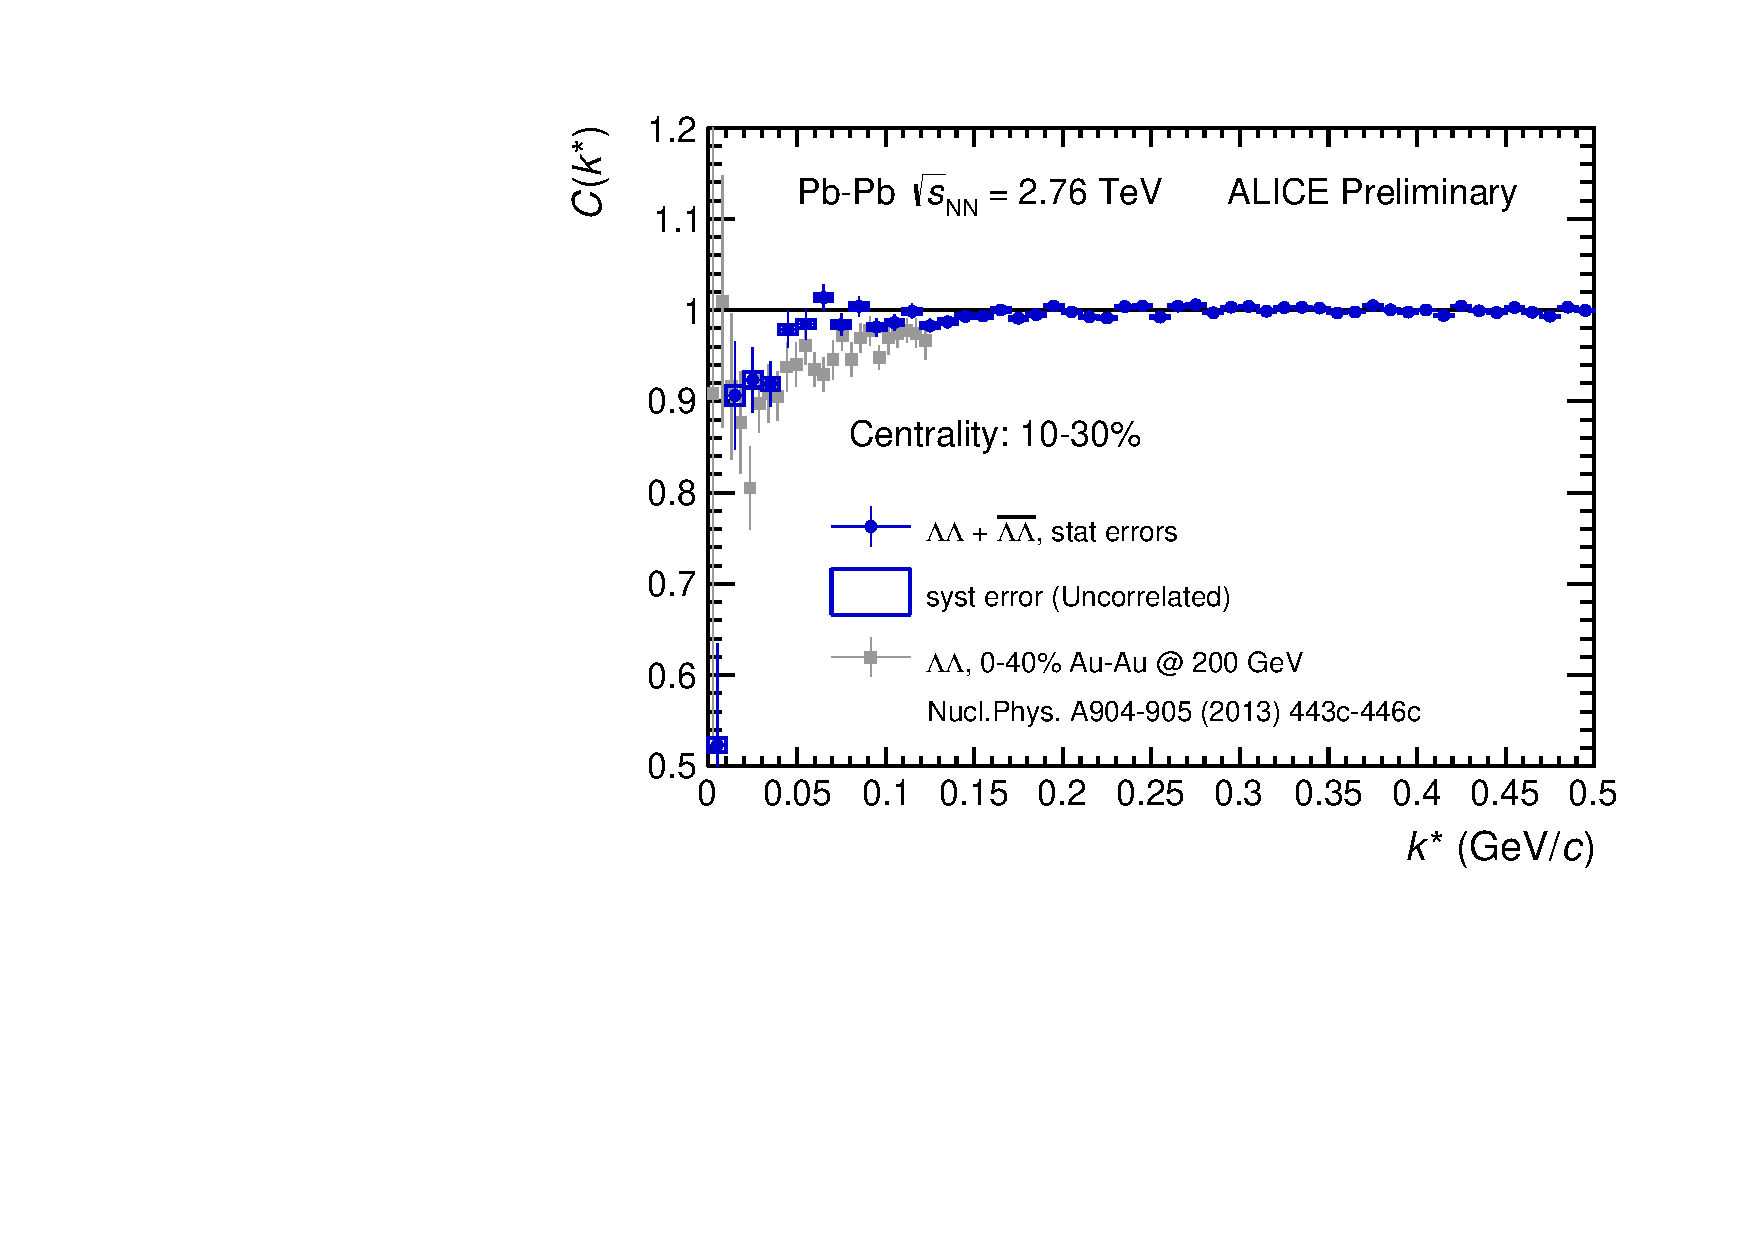
\includegraphics[width=36pc]{Figures/2014-05-11-CfLLAA-1030-CommentCorrections-WithSTAR.pdf}
\caption[$\Lambda\Lambda + \bar{\Lambda}\bar{\Lambda}$ correlation function for the 10-30\% centrality range]{$\Lambda\Lambda + \bar{\Lambda}\bar{\Lambda}$ correlation function for the 10-30\% centrality range with statistical and systematic errors.  A dip at low $k^*$ is seen which is expected from quantum interference.  Preliminary STAR data for $\Lambda\Lambda$ is shown for comparison.}
\label{fig:AppendixCFLamLamALamALam1030STAR}
\end{figure}
\begin{figure}[hbtp]
\includegraphics[width=36pc]{Figures/2014-05-11-CfLLAA-3050-CommentCorrections.pdf}
\caption[$\Lambda\Lambda + \bar{\Lambda}\bar{\Lambda}$ correlation function for the 30-50\% centrality range]{$\Lambda\Lambda + \bar{\Lambda}\bar{\Lambda}$ correlation function for the 30-50\% centrality range with statistical and systematic errors.  A hint of a dip at low $k^*$ may be seen, which would be expected from quantum interference.}
\label{fig:AppendixCFLamLamALamALam3050}
\end{figure}

%\subsection{Plots currently approved}


\bibliographystyle{unsrt}
\bibliography{bibfile}





%\end{document}